% SI - Figure 1 Example route with data
\begin{figure}[htb]
\centering
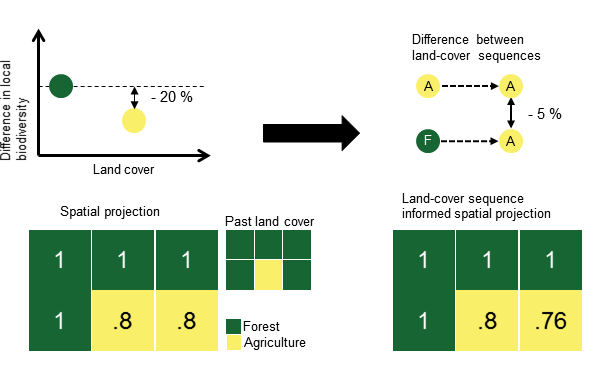
\includegraphics[width=1\textwidth]{chapter5/SI01}
\caption{Annual Landsat composite for a single year (2018) and route (RTENO: \texttt{89020}, Routename: \texttt{Wapato} in the State of Washington) showing the month with the greenest EVI value in the period 20\textsuperscript{th} March to 20\textsuperscript{th} June. }
\label{SI05_01}
\end{figure}

% SI - Figure 2 Missing data
\begin{figure}[htb]
\centering
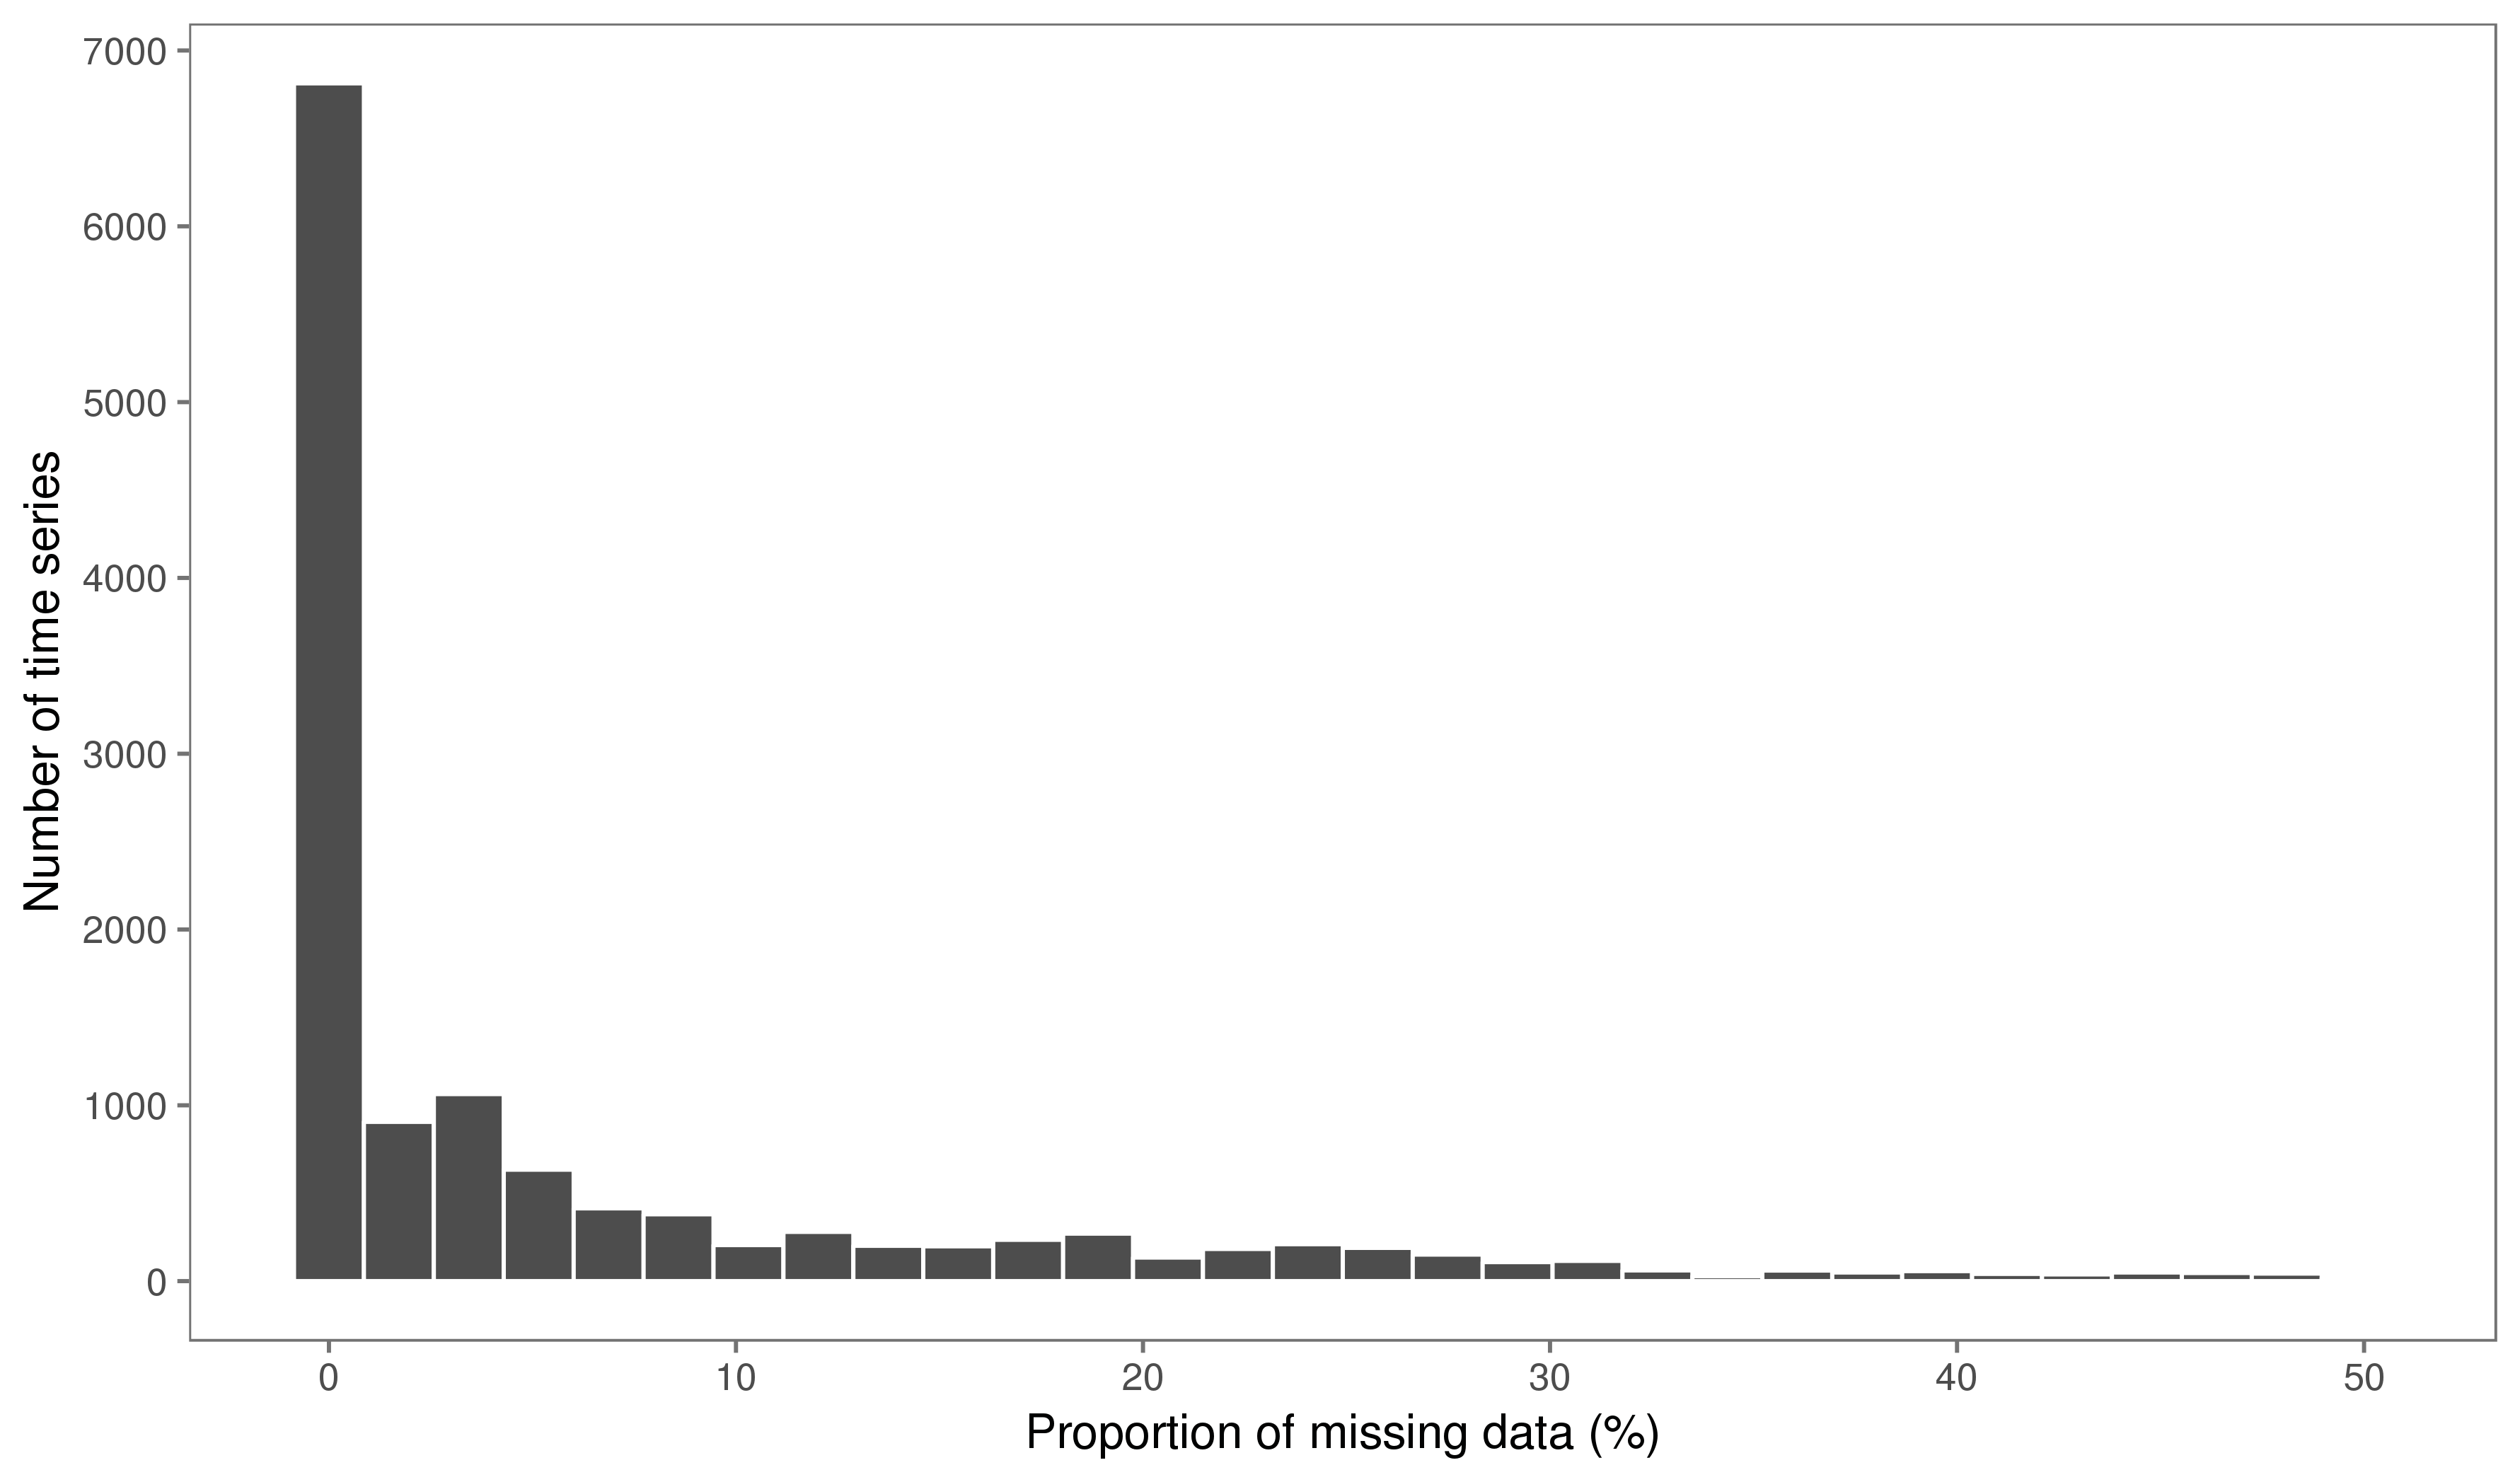
\includegraphics[width=1\textwidth]{chapter5/SI02}
\caption{(\textbf{a}) Average proportion of missing Landsat data across years for all routes with the median (1.06\%) indicated (dotted line). (\textbf{b}) Map showing each BBS Route coloured by the average proportion (\%) of missing data across years.}
\label{SI05_02}
\end{figure}

% SI - Figure 3-4 Model checks
\begin{figure}[htb]
\centering
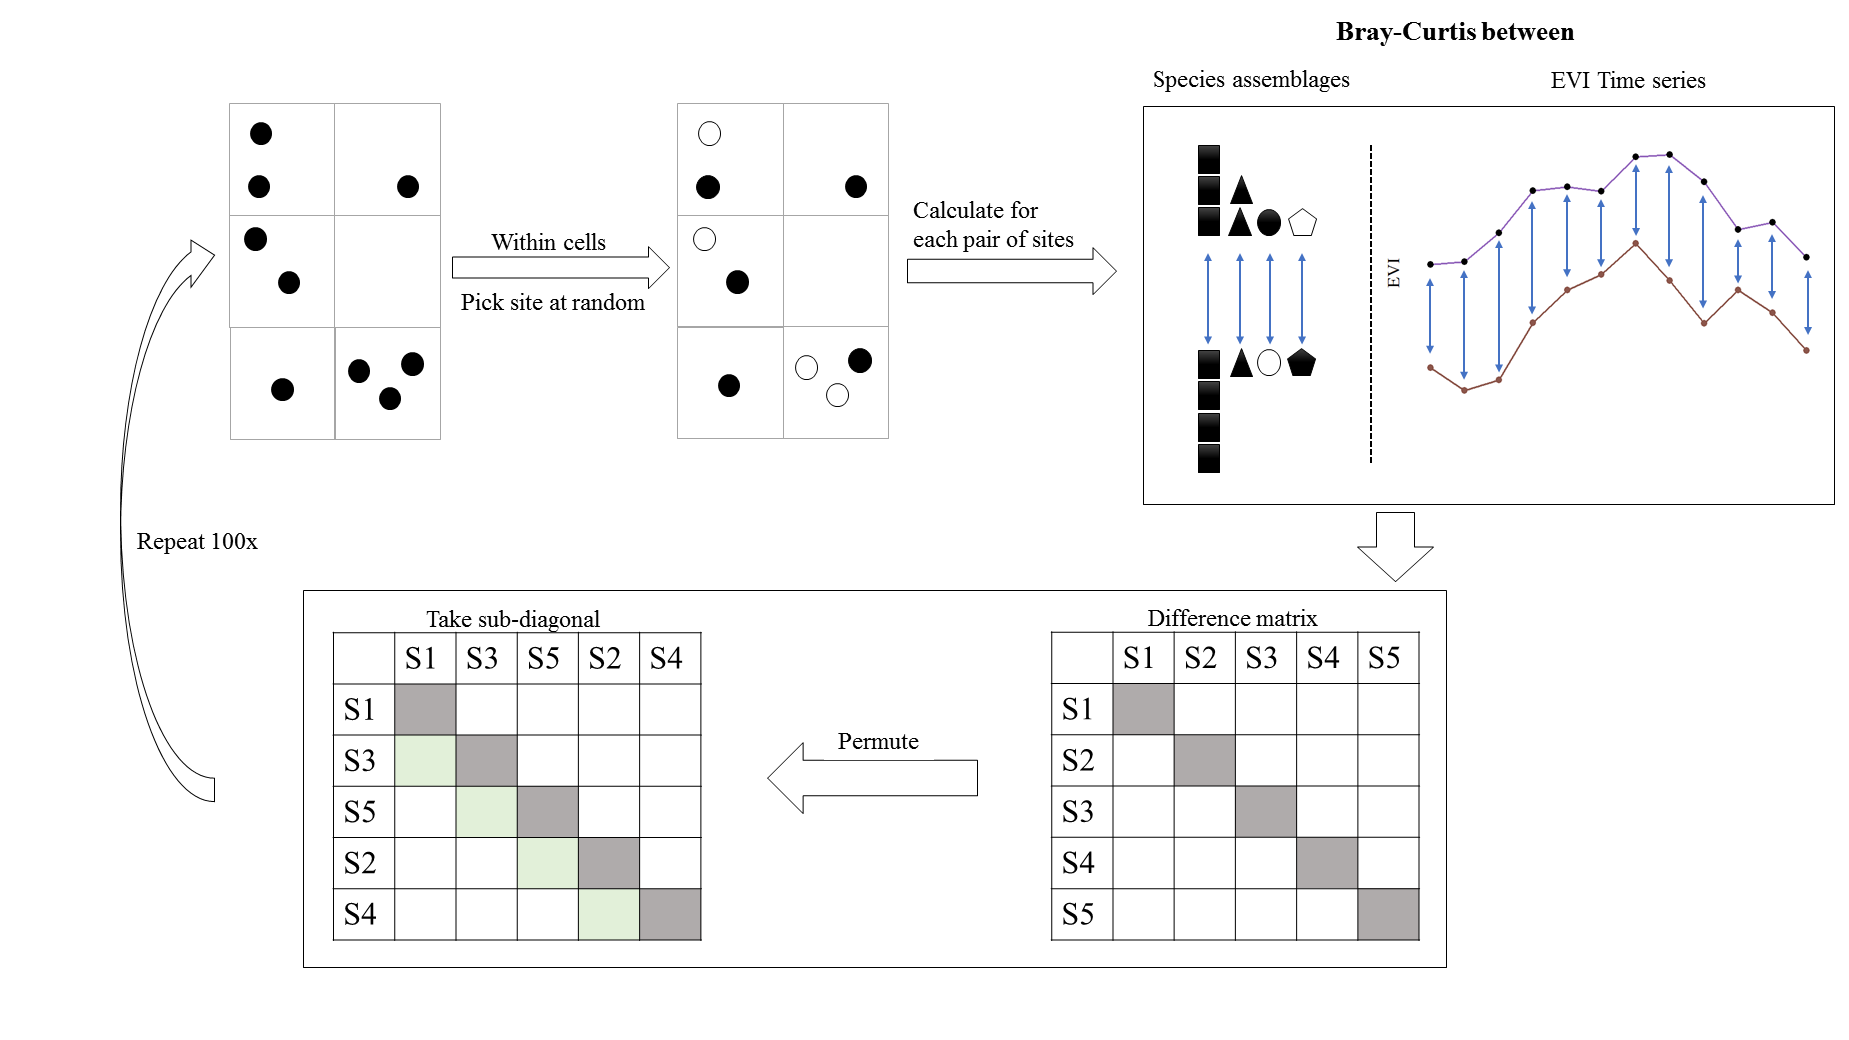
\includegraphics[width=.9\textwidth]{chapter5/SI03}
\caption{Model diagnostics of the full model (see \ref{C05_0205}) for the geometric mean of relative abundances (GM).}
\label{SI05_03}
\end{figure}

\begin{figure}[htb]
\centering
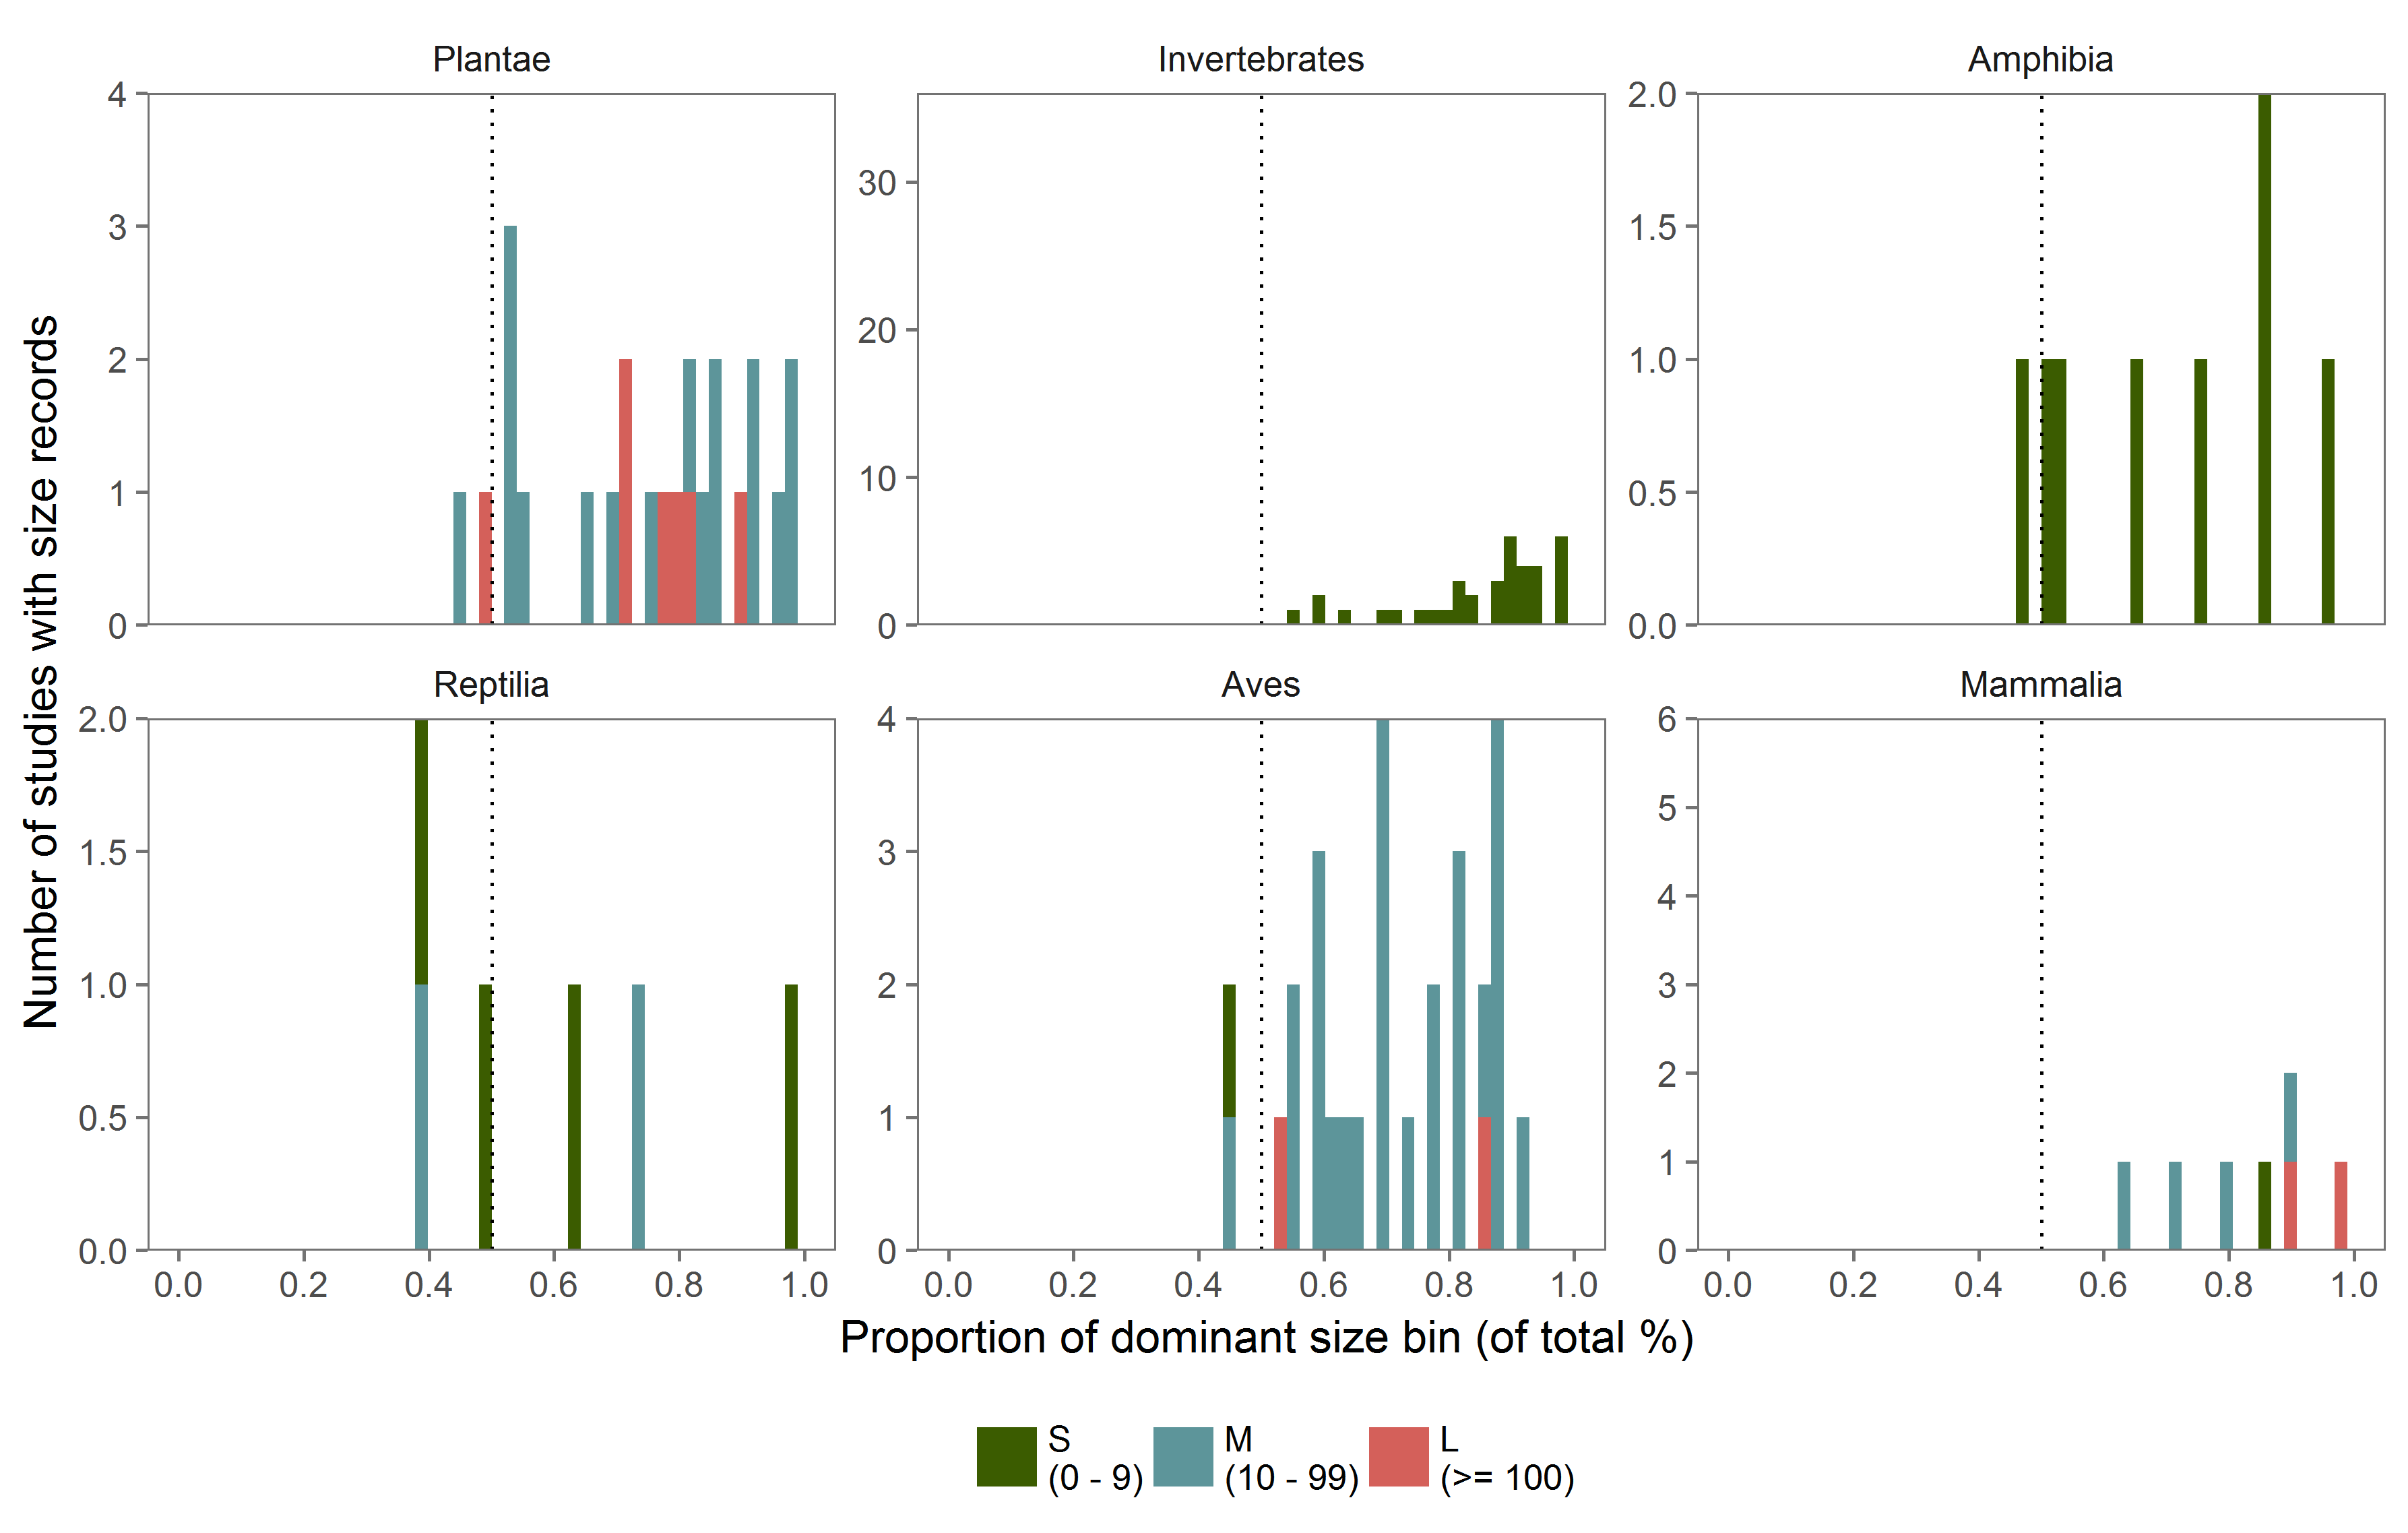
\includegraphics[width=.9\textwidth]{chapter5/SI04}
\caption{Model diagnostics of the full model (see \ref{C05_0205}) for the progressive Bray-Curtis index (pBC).}
\label{SI05_04}
\end{figure}

% SI - Figure 5 Annual trends
\begin{figure}[htb]
\centering
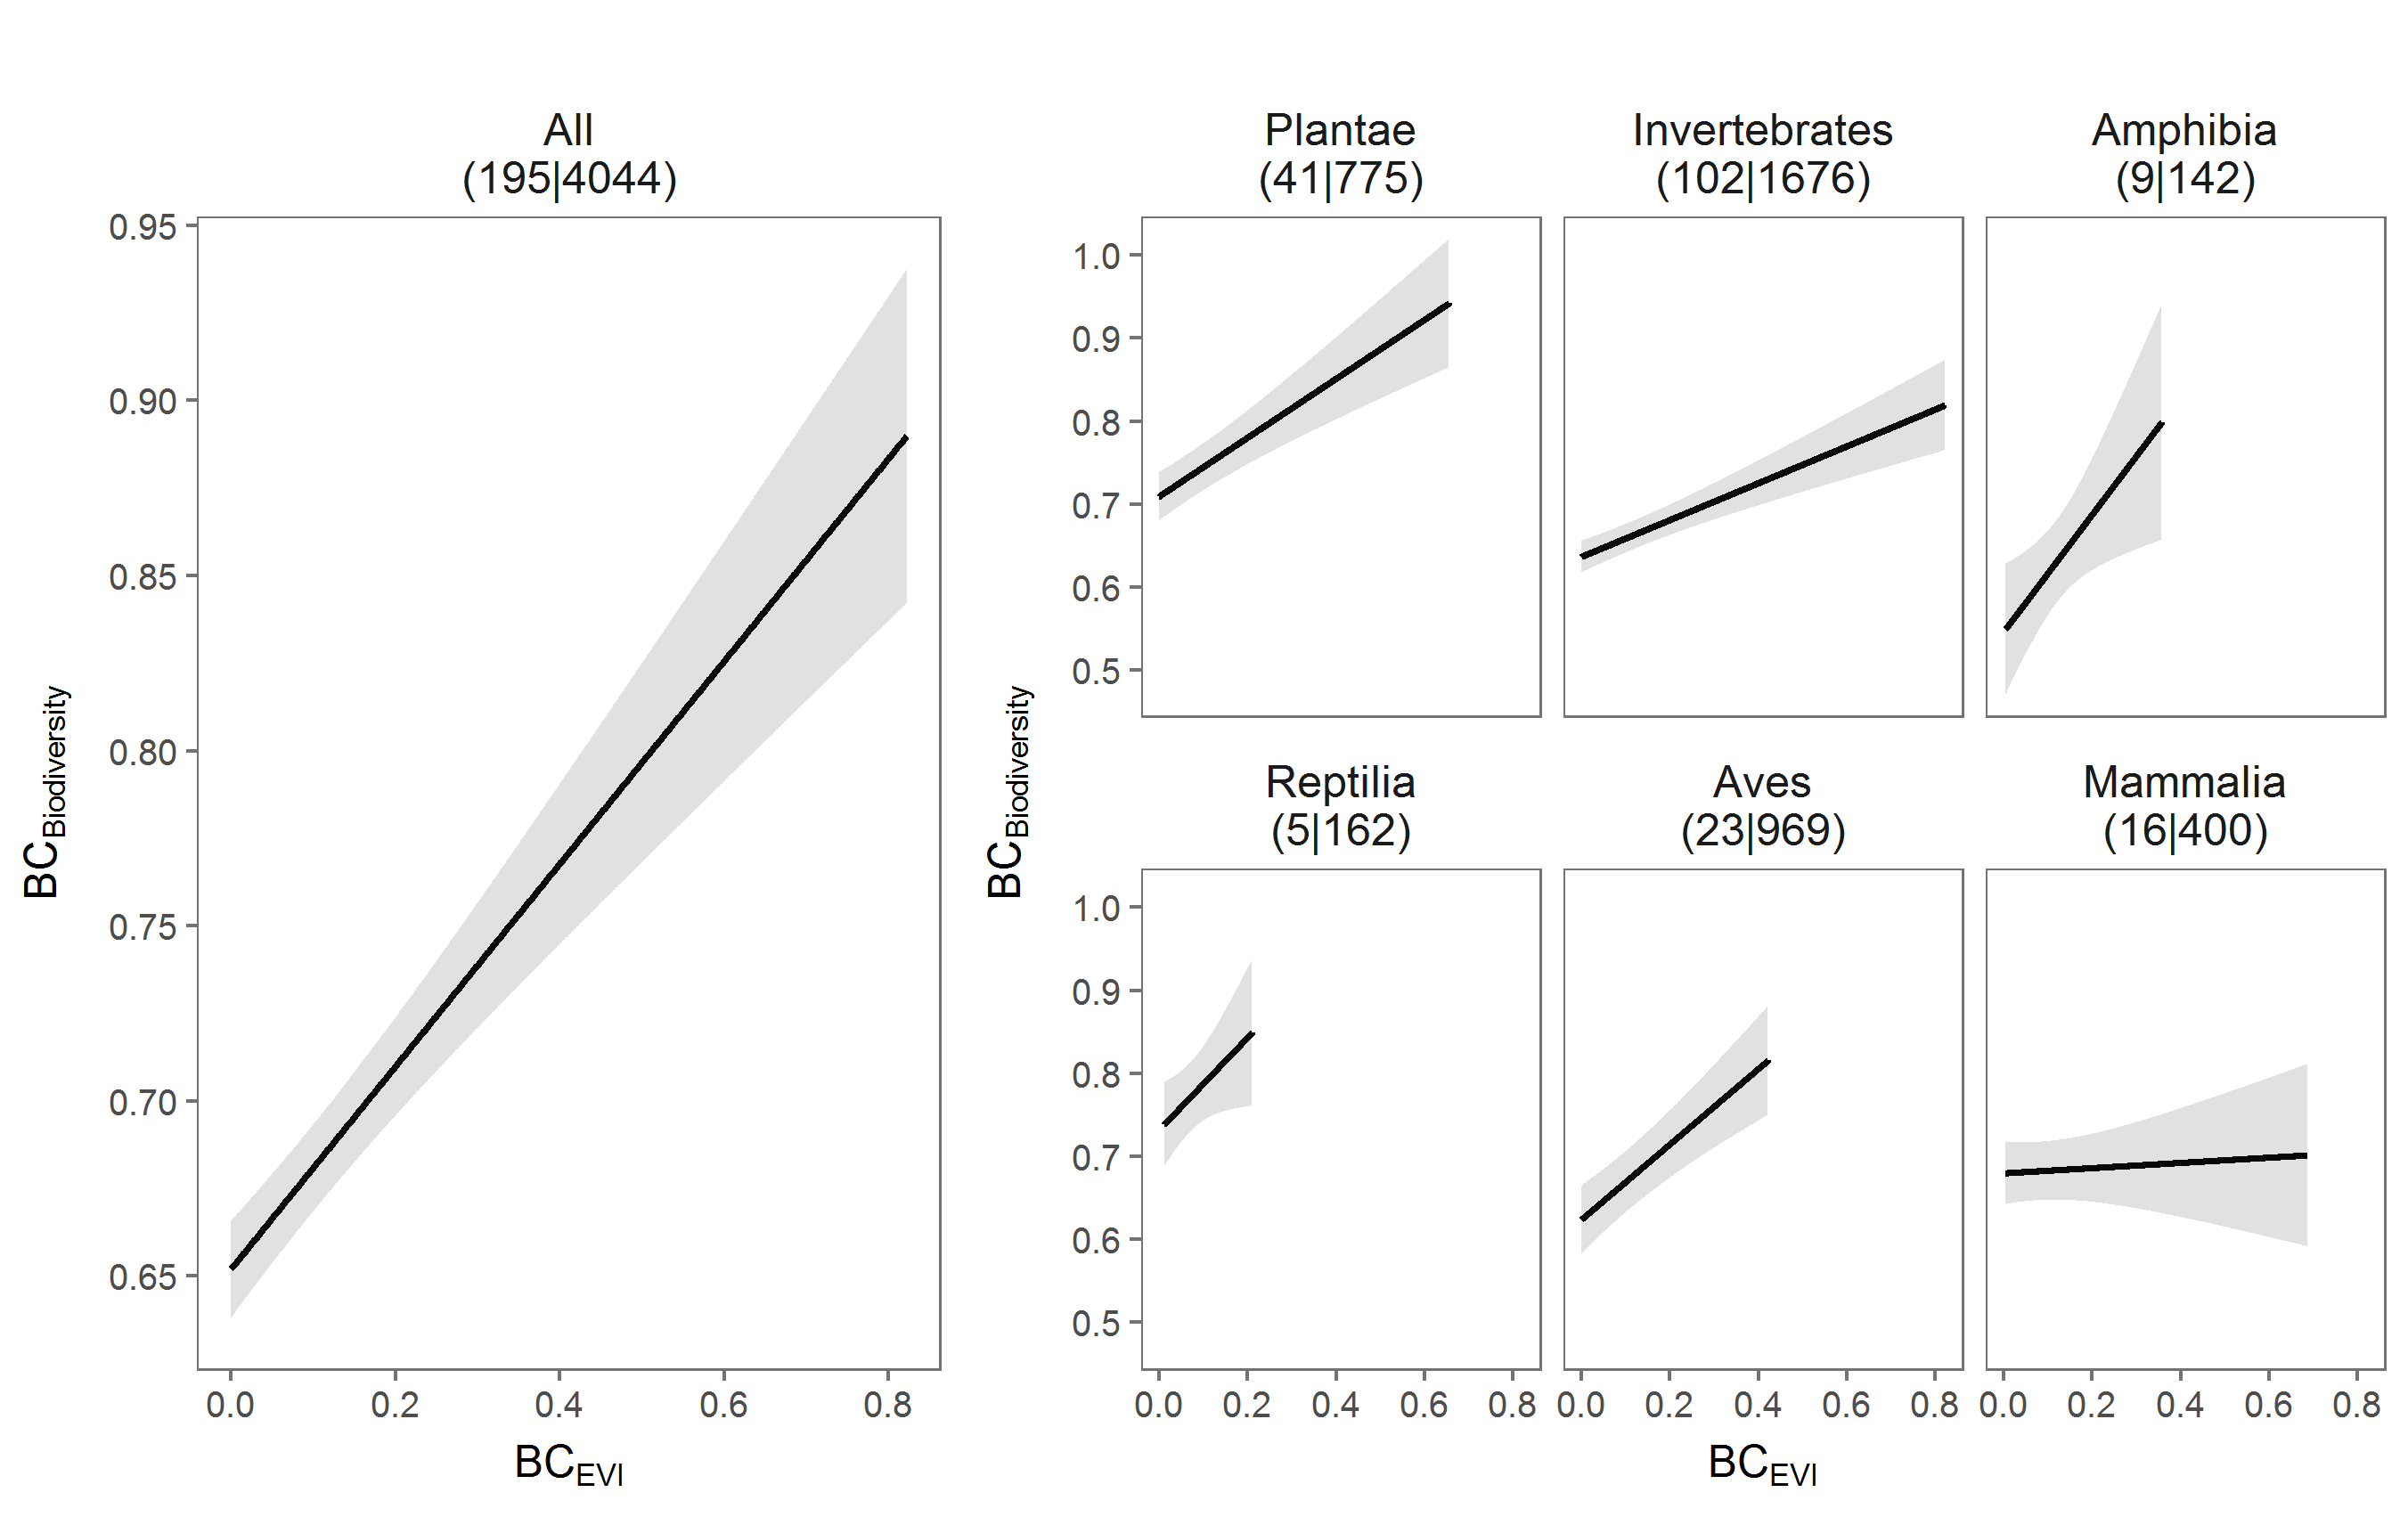
\includegraphics[width=1\textwidth]{chapter5/SI05}
\caption{Average trend in the (\textbf{a}) GM and (\textbf{b}) the pBC over the considered monitoring period (1984-2017) and across all 2745 BBS routes. Error margins show $\pm$ 1 standard error.}
\label{SI05_05}
\end{figure}

% SI - Figure 6 Map with total number of changes
\begin{figure}[htb]
\centering
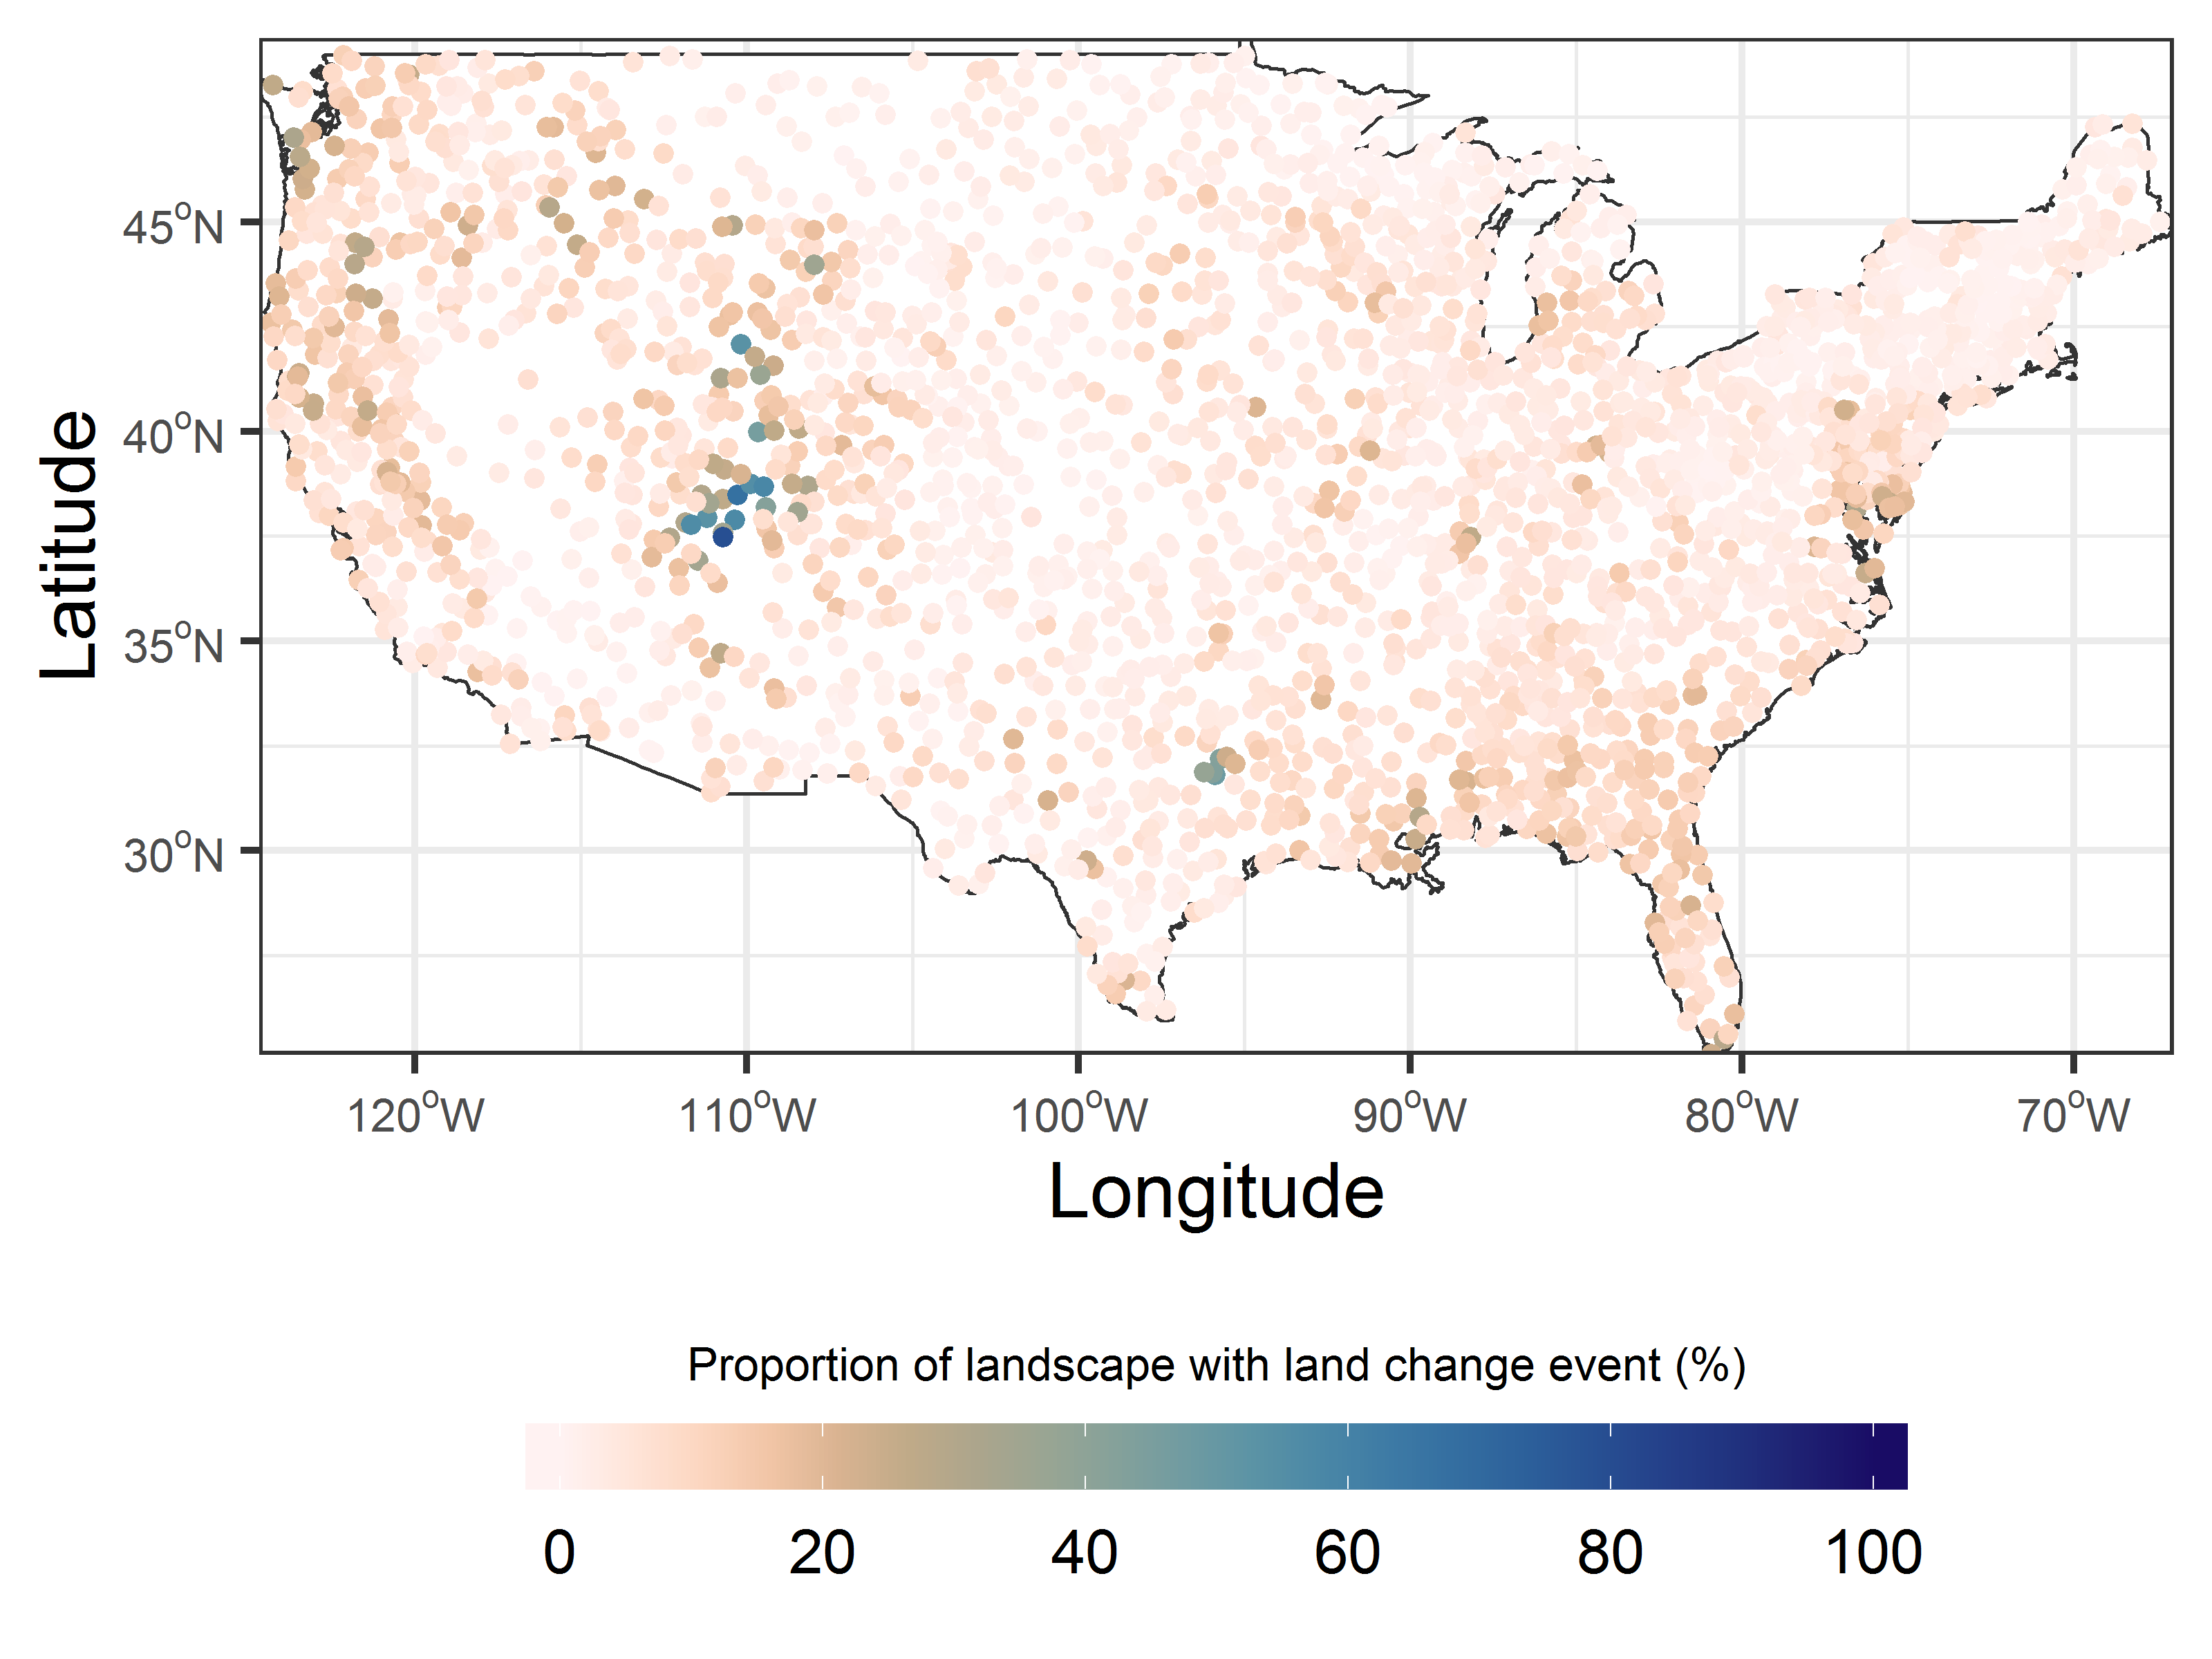
\includegraphics[width=.9\textwidth]{chapter5/SI06}
\caption{The centroids of all BBS routes (see methods) coloured by the total proportion of the landscape that had at least one land change event in the period 1984 to 2017.}
\label{SI05_06}
\end{figure}

% SI - Figure 7 Map with trend of land changes
\begin{figure}[htb]
\centering
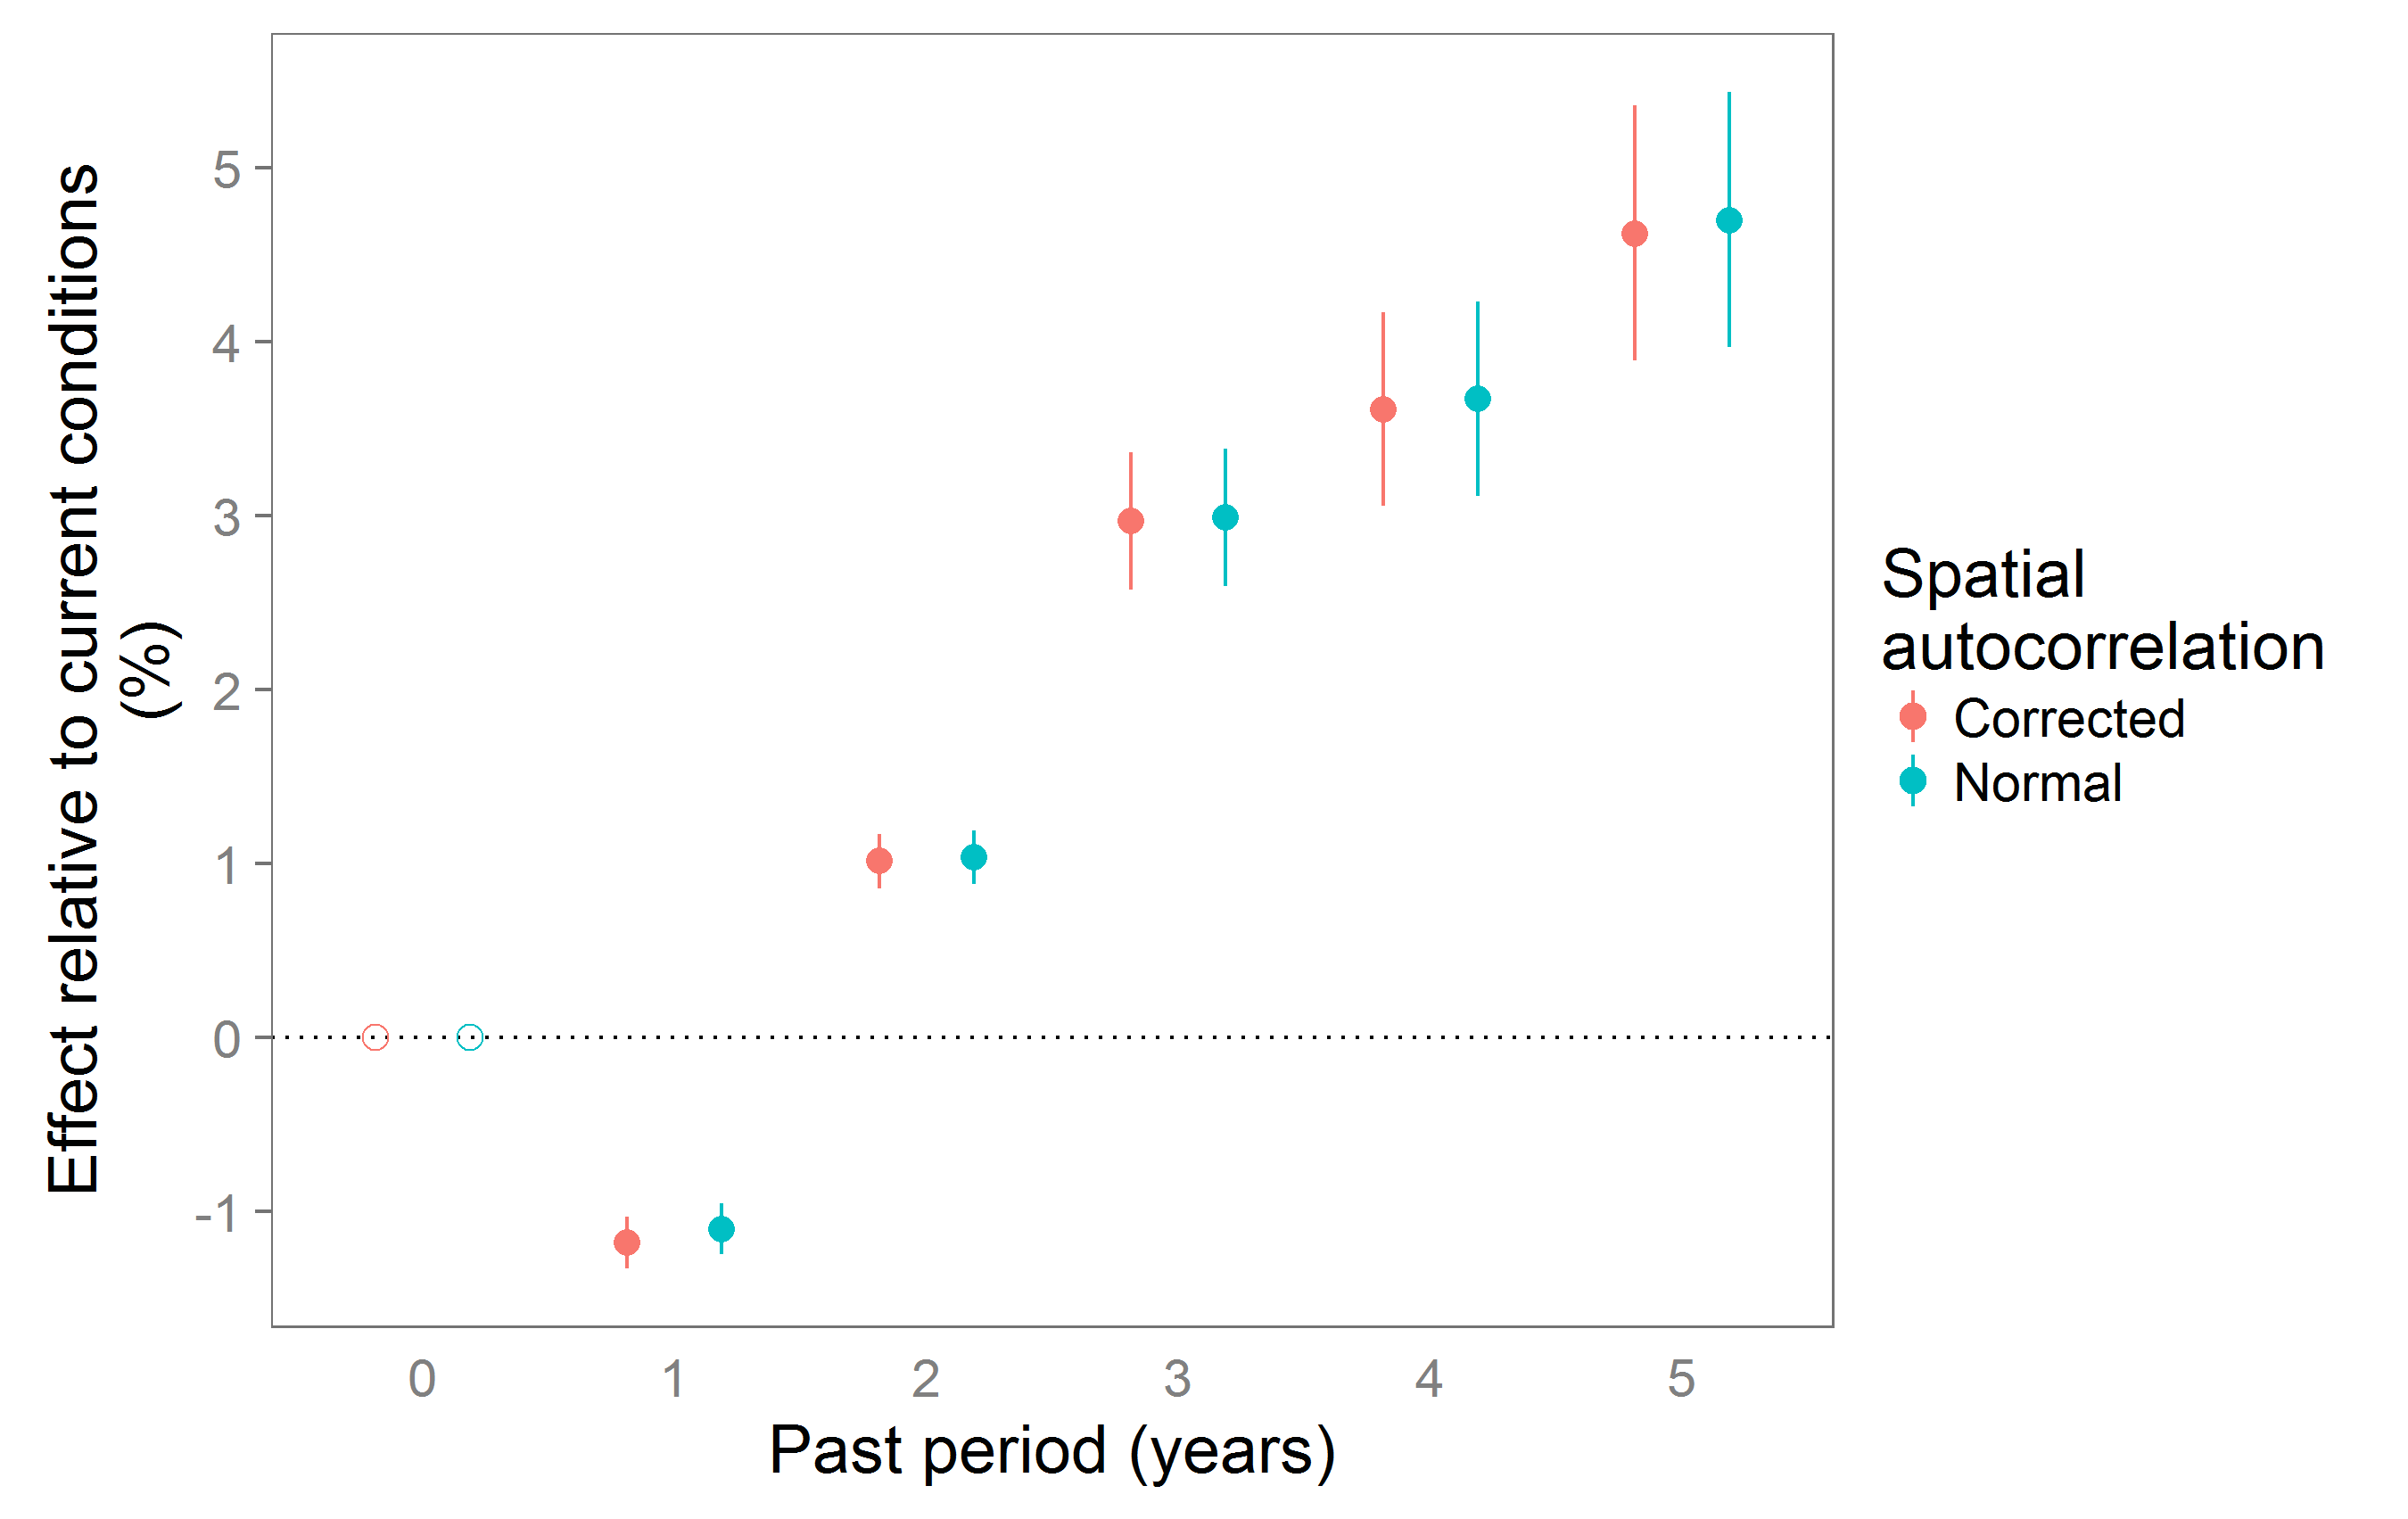
\includegraphics[width=.9\textwidth]{chapter5/SI07}
\caption{Robust annual linear trends in the proportion of land with an abrupt shift in magnitude (loss + gain) across all landscapes surrounding BBS routes. The most extreme estimate (99\% lower and upper limits) were excluded from this visualization (N = 56). }
\label{SI05_07}
\end{figure}

% SI - Figure 8 Trend of land change
\begin{figure}[htb]
\centering
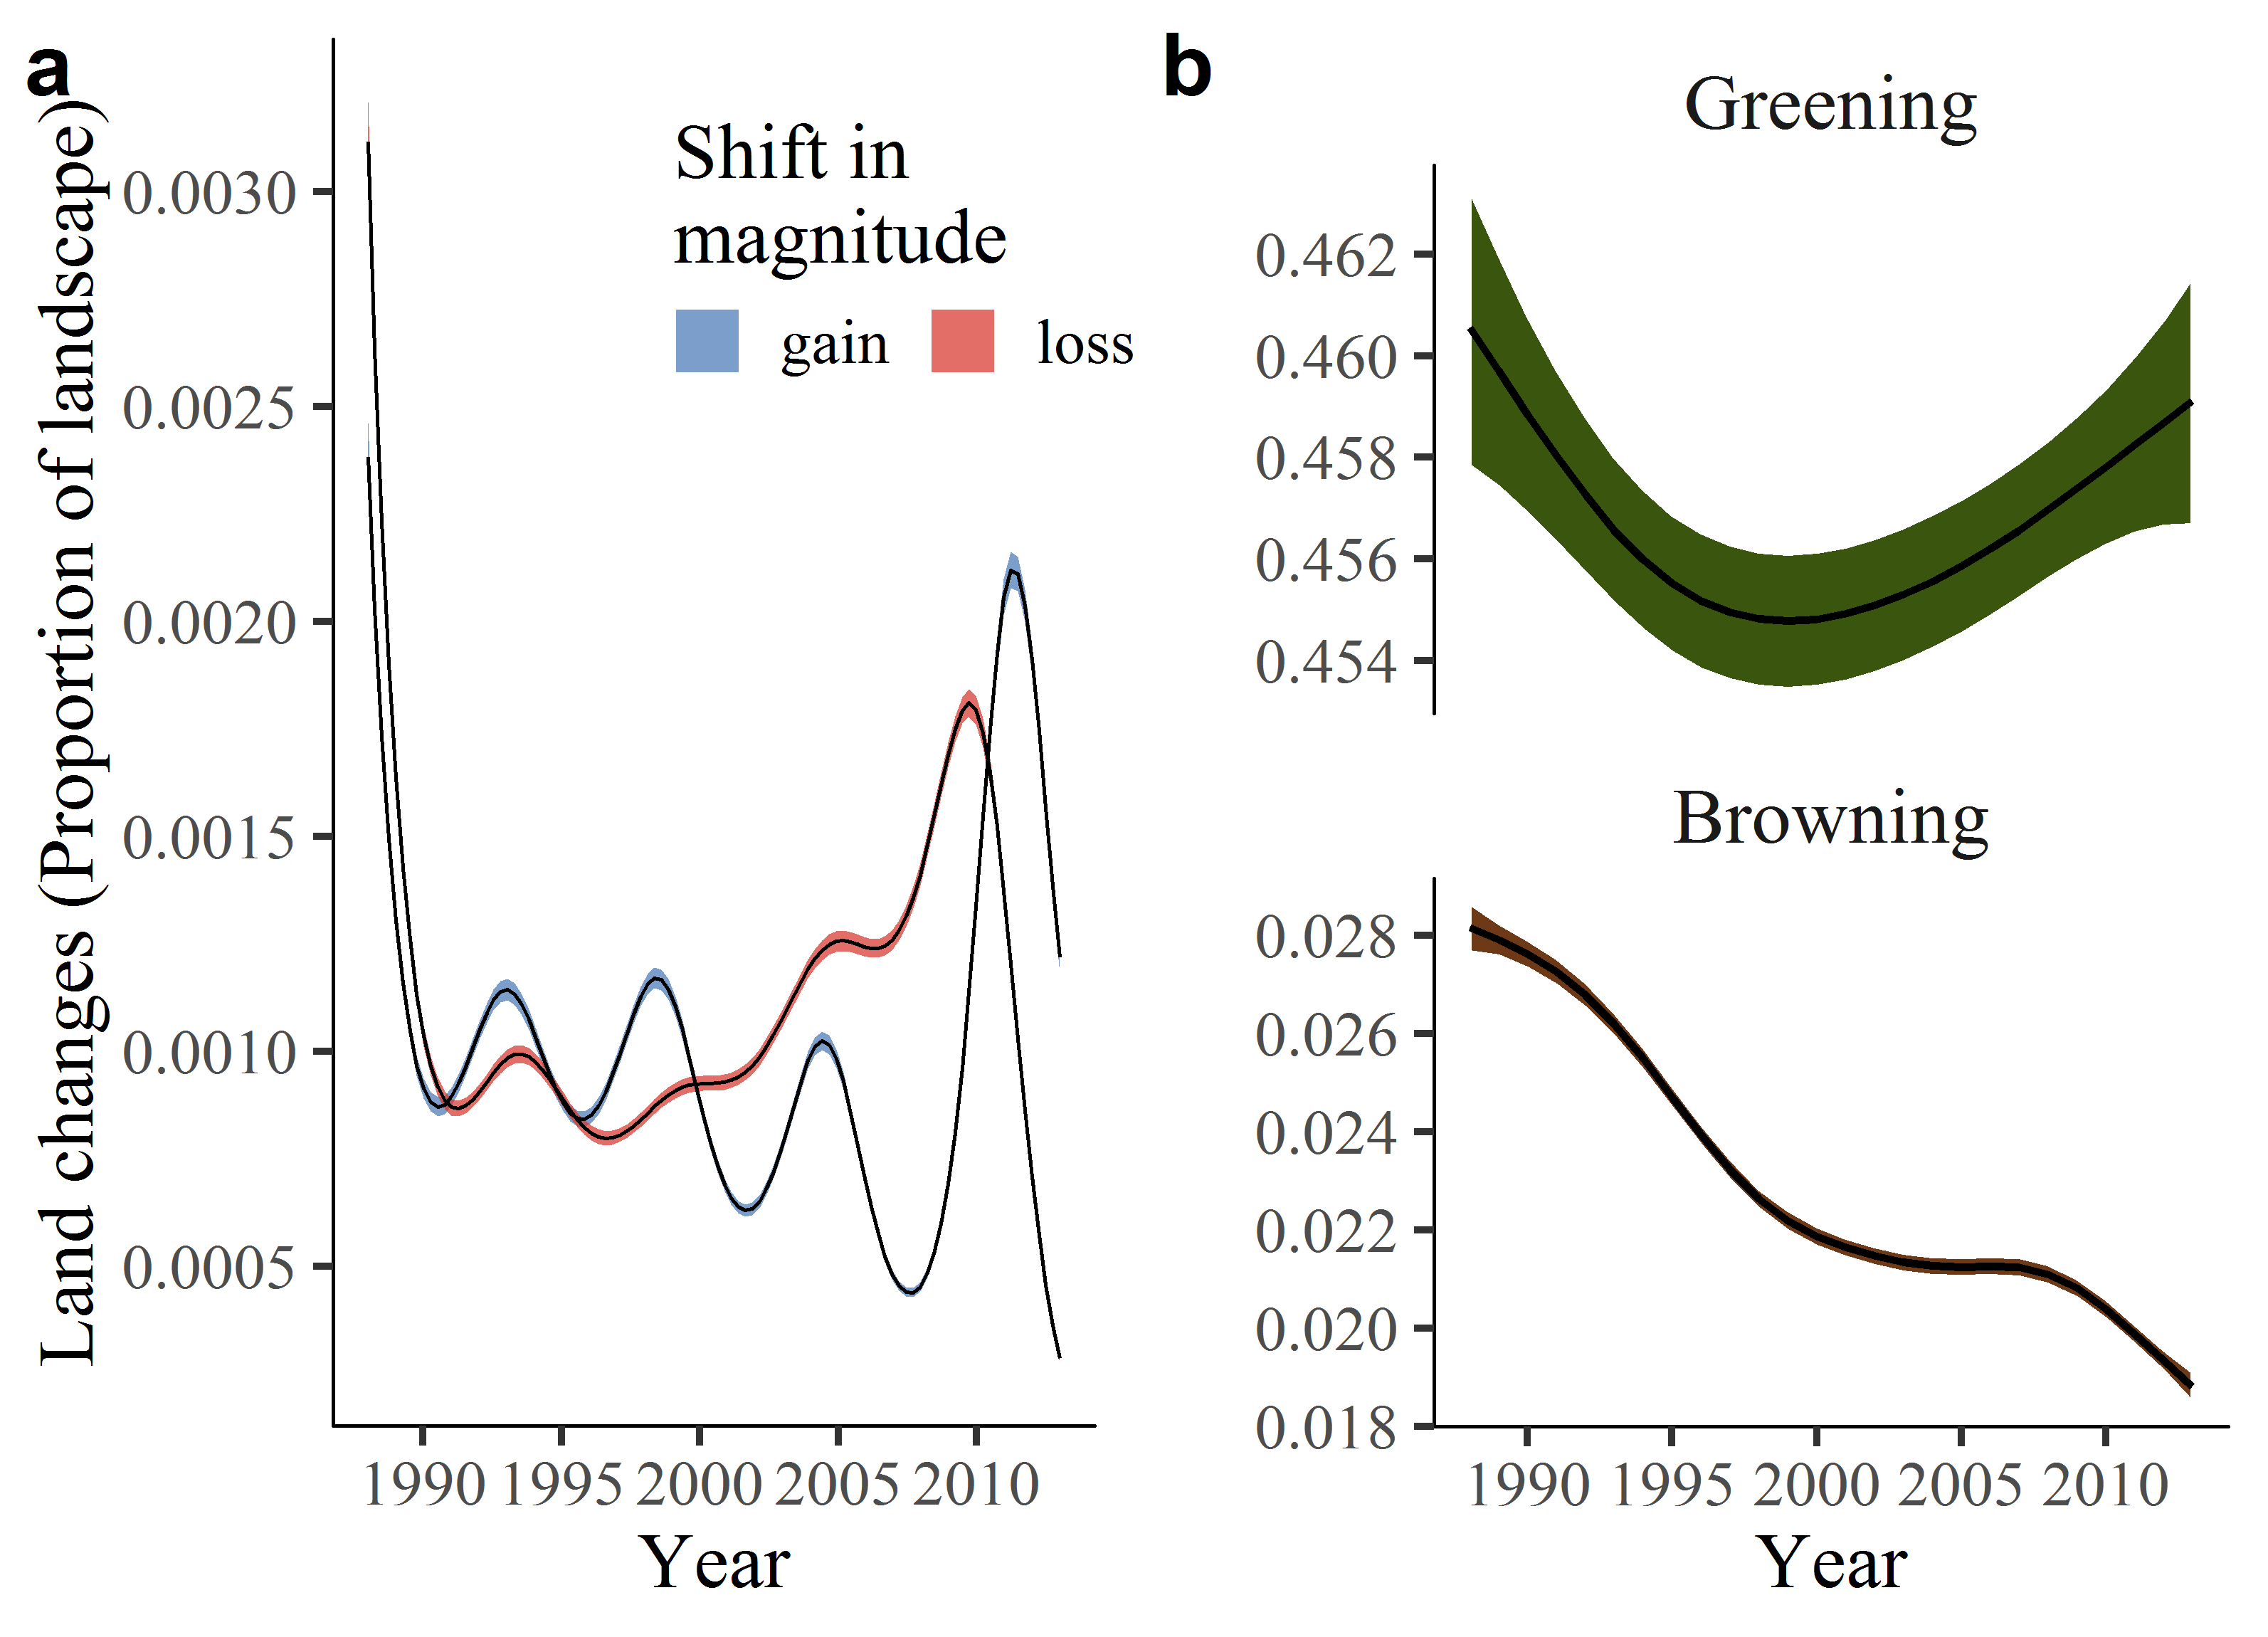
\includegraphics[width=1\textwidth]{chapter5/SI08}
\caption{Average trend of land changes with abrupt shift in (\textbf{a}) magnitude or (\textbf{b}) shift in trend as predicted by a GAM that includes a non-linear term for year only. Error bands show the fitted standard error.}
\label{SI05_08}
\end{figure}

% SI - Figure 9 Pairwise correlation plot
\begin{figure}[htb]
\centering
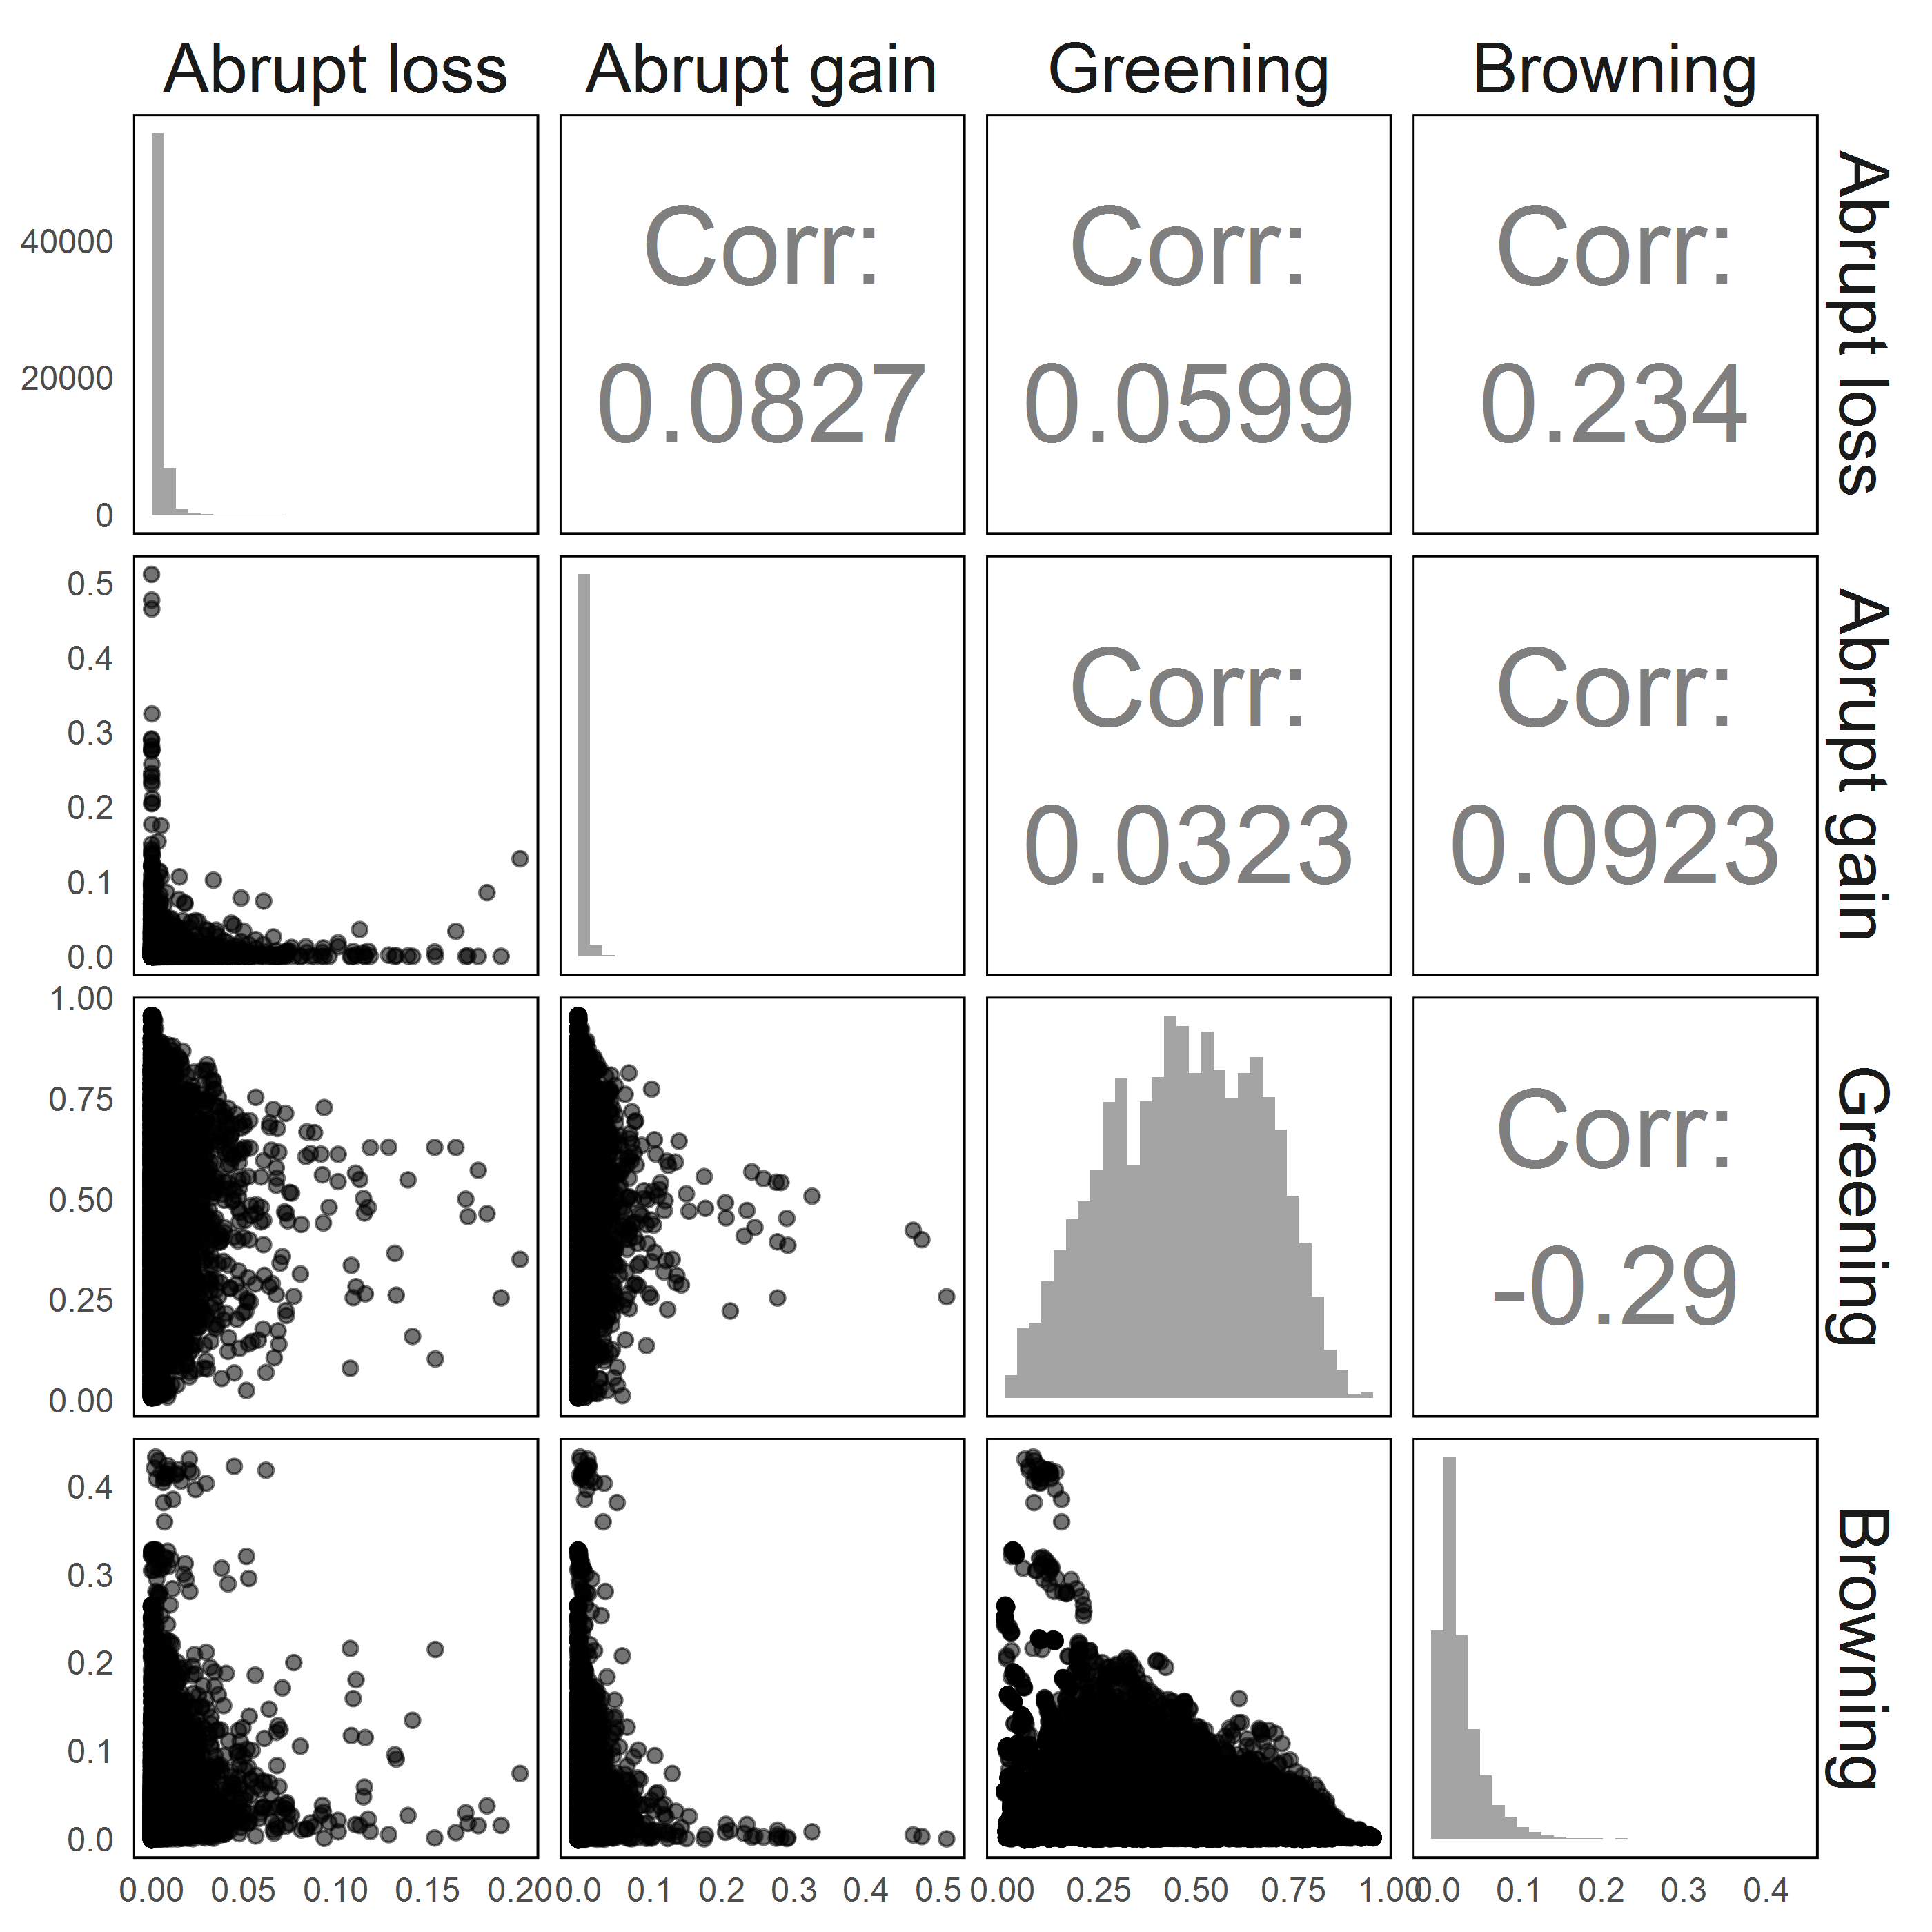
\includegraphics[width=1\textwidth]{chapter5/SI09}
\caption{Pairwise correlation plot plot between the proportion of land changes with abrupt shifts in magnitude (gains and losses in photosynthetic activity) and trend (greening and browning). Text in upper triangle shows the Pearson correlation coefficients.}
\label{SI05_09}
\end{figure}

% SI - Figure 10 Change per ecoregion
\begin{figure}[htb]
\centering
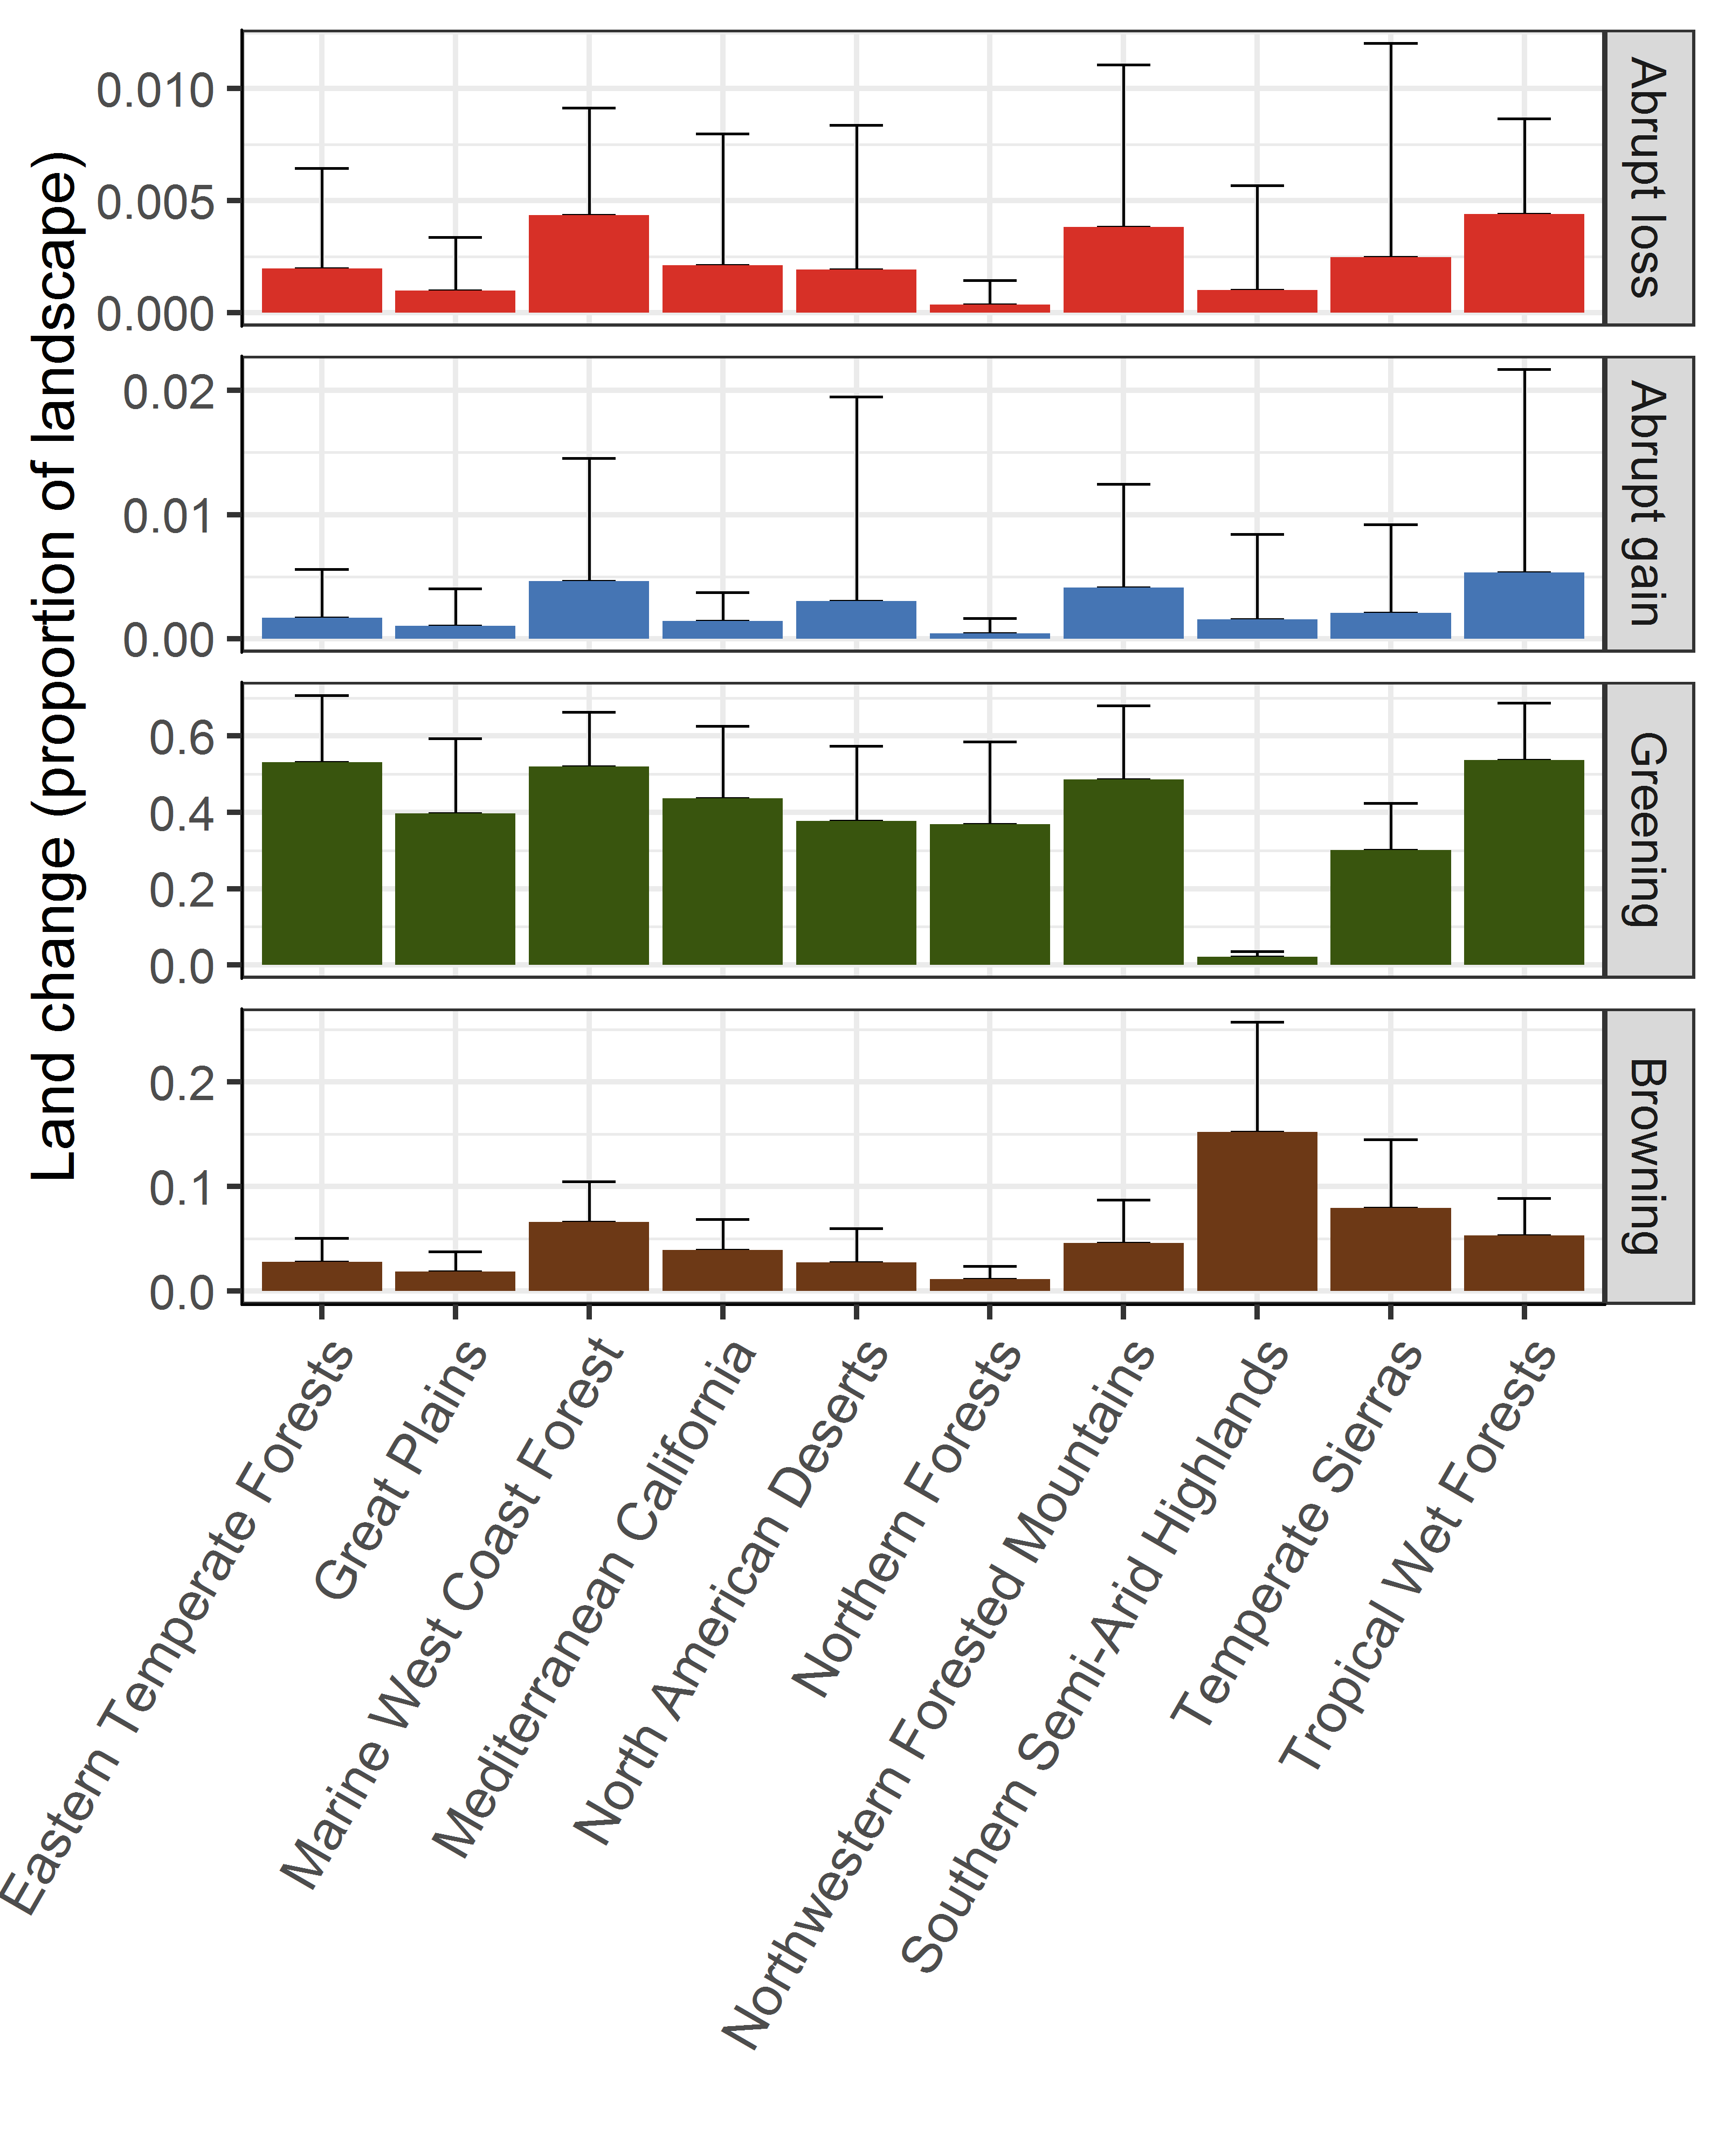
\includegraphics[width=1\textwidth]{chapter5/SI10}
\caption{Average proportion of landscape-wide land changes \textendash\ shifts in magnitude, \eg abrupt losses and gains, and shift in trends, \eg greening and browning \textendash\ across 10 US ecoregions. Error bars show the calculated standard deviation. Colours as in Appendix figure \ref{SI05_08}.}
\label{SI05_10}
\end{figure}

% SI - Figure 11 Partial effects of local factors
\begin{figure}[htb]
\centering
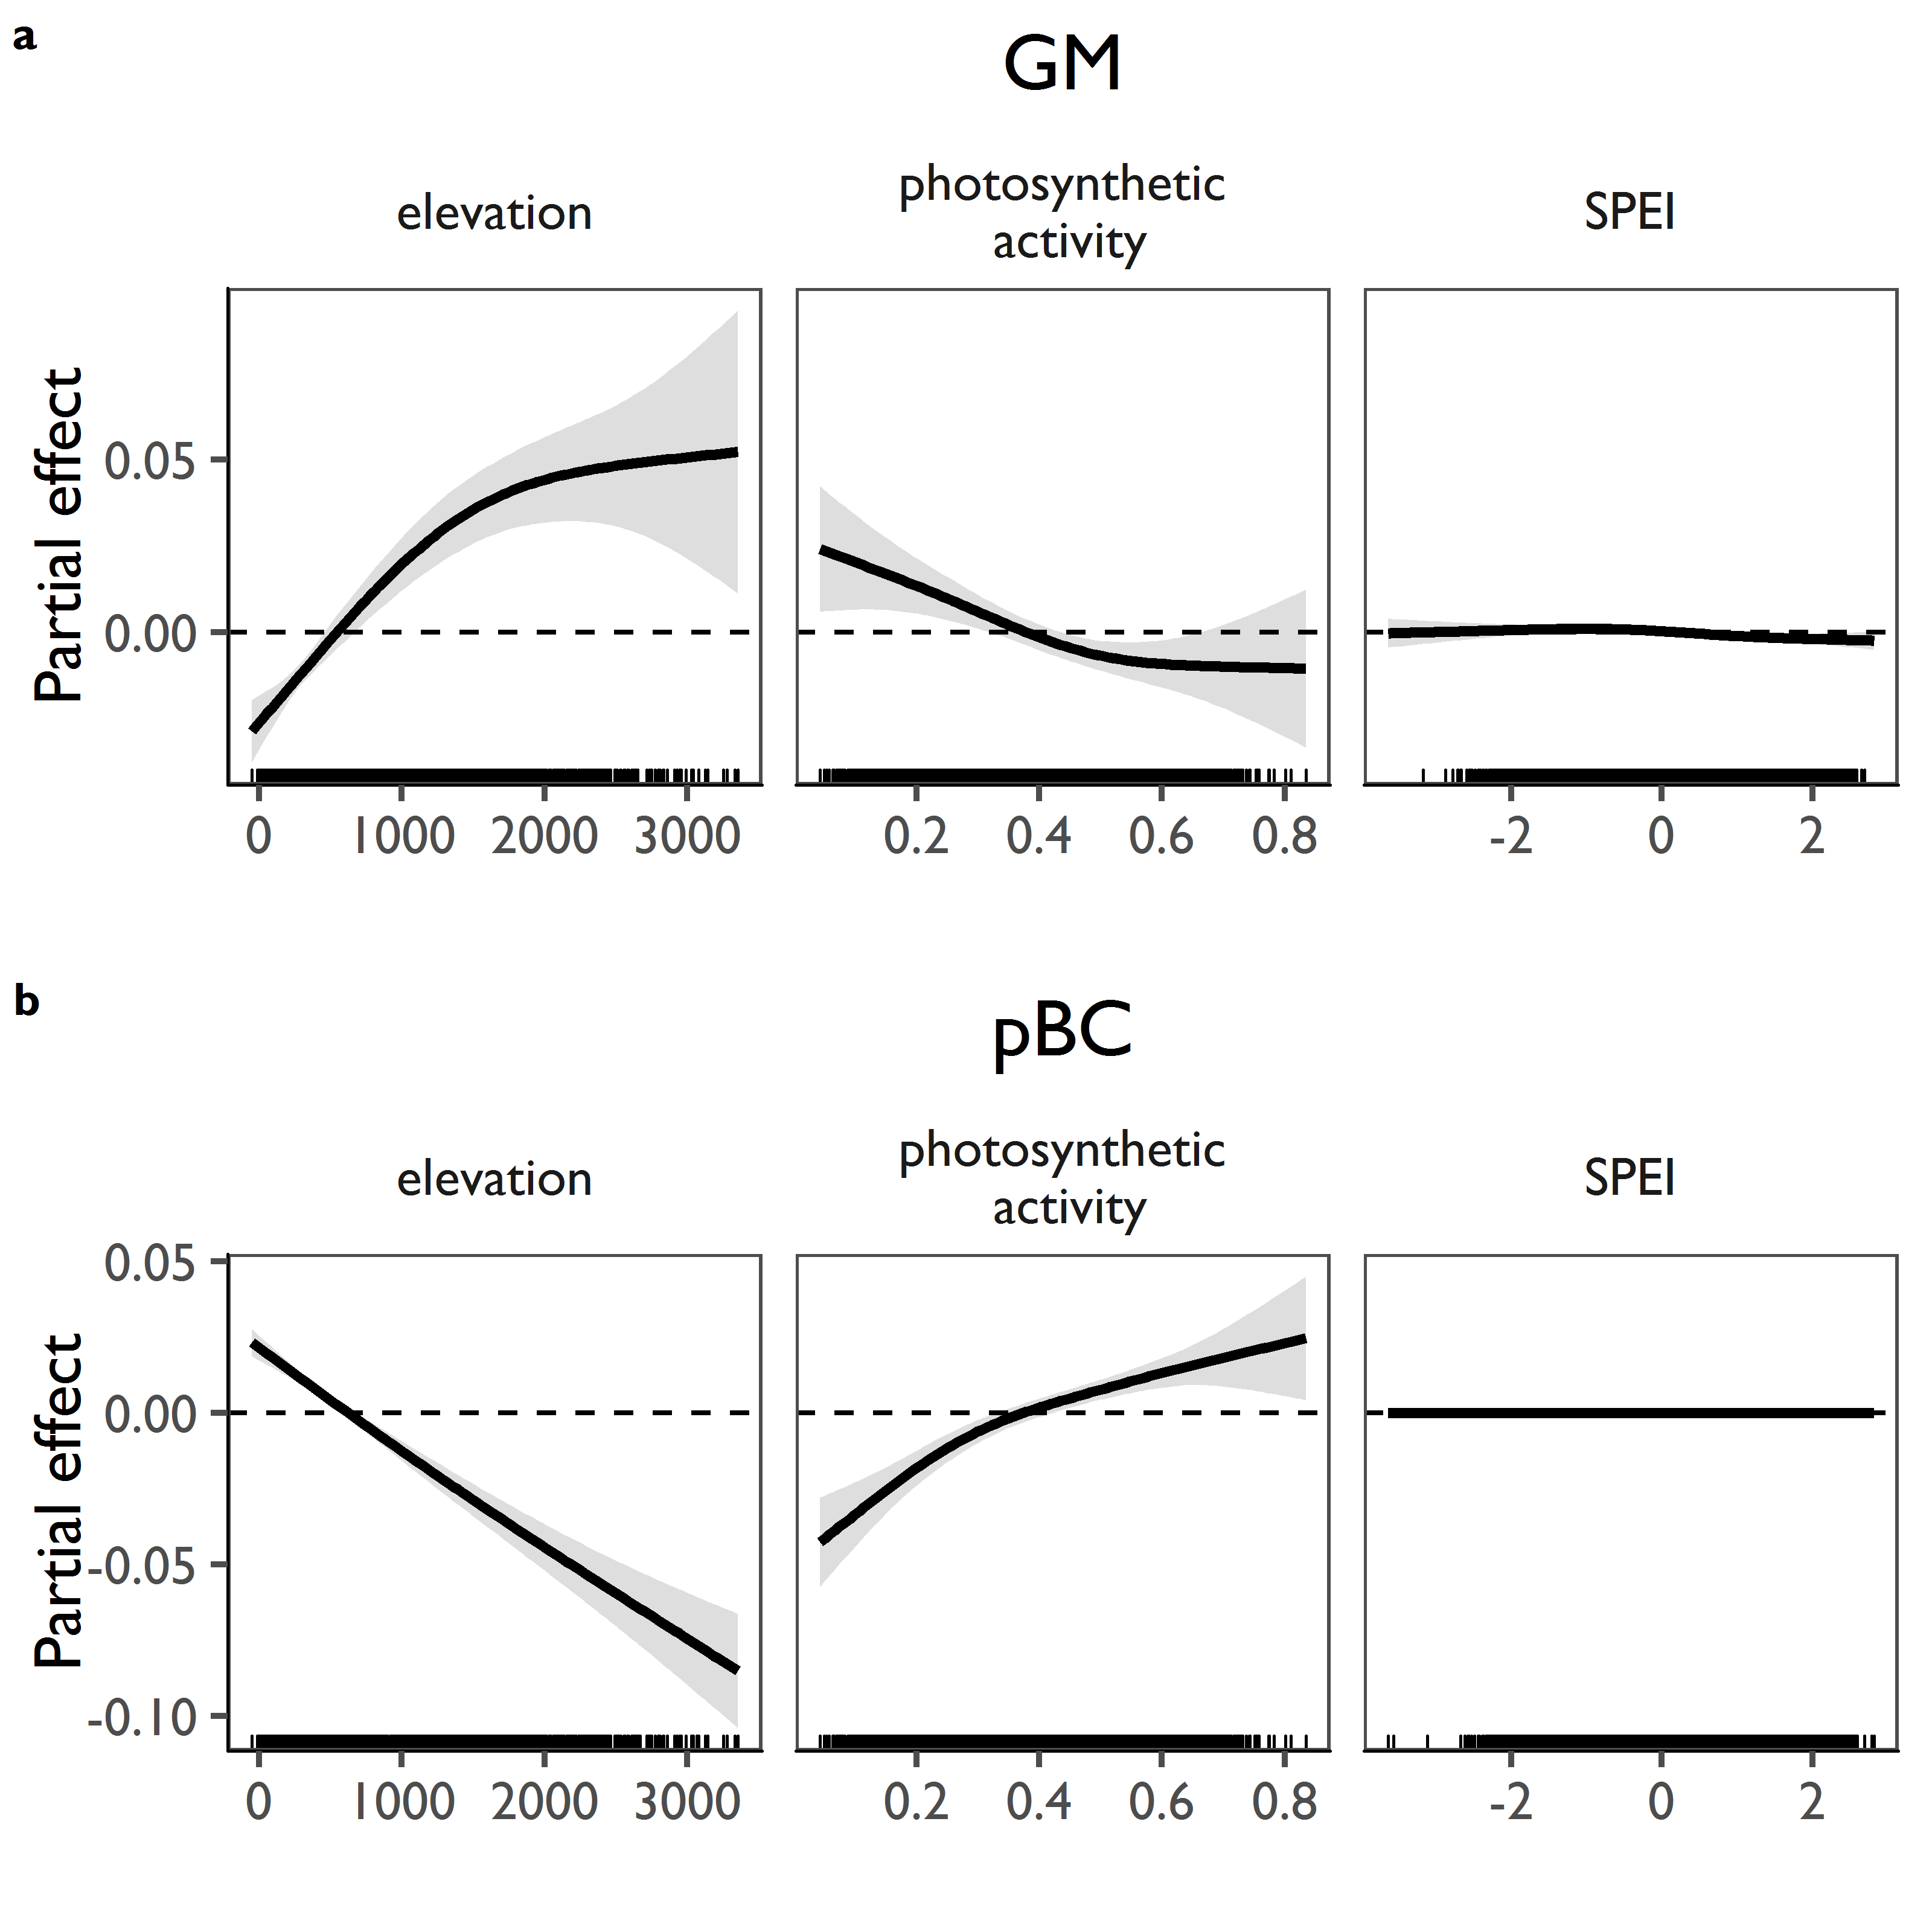
\includegraphics[width=1\textwidth]{chapter5/SI11}
\caption{Estimated partial effect of f\textunderscript{local} variables (see methods \ref{C05_02}) on (\textbf{a}) GM and (\textbf{b}) pBC. The Y-axis shows the annual change in GM or pBC for each unit of the f\textunderscript{local} variables. Photosynthetic activity is measured as average EVI across the entire landscape and time period (1984-2017). SPEI stands for the Standardised Precipitation-Evapotranspiration Index \citep{Vicente-Serrano2010}. Flat lines without uncertainty indicate that the term was penalized out during the model fitting and therefore had no additive effect on the biodiversity measure. Error margins show the estimated standard error of the partial effects.
}
\label{SI05_11}
\end{figure}

% SI - Figure 12 Trends of traits
\begin{figure}[htb]
\centering
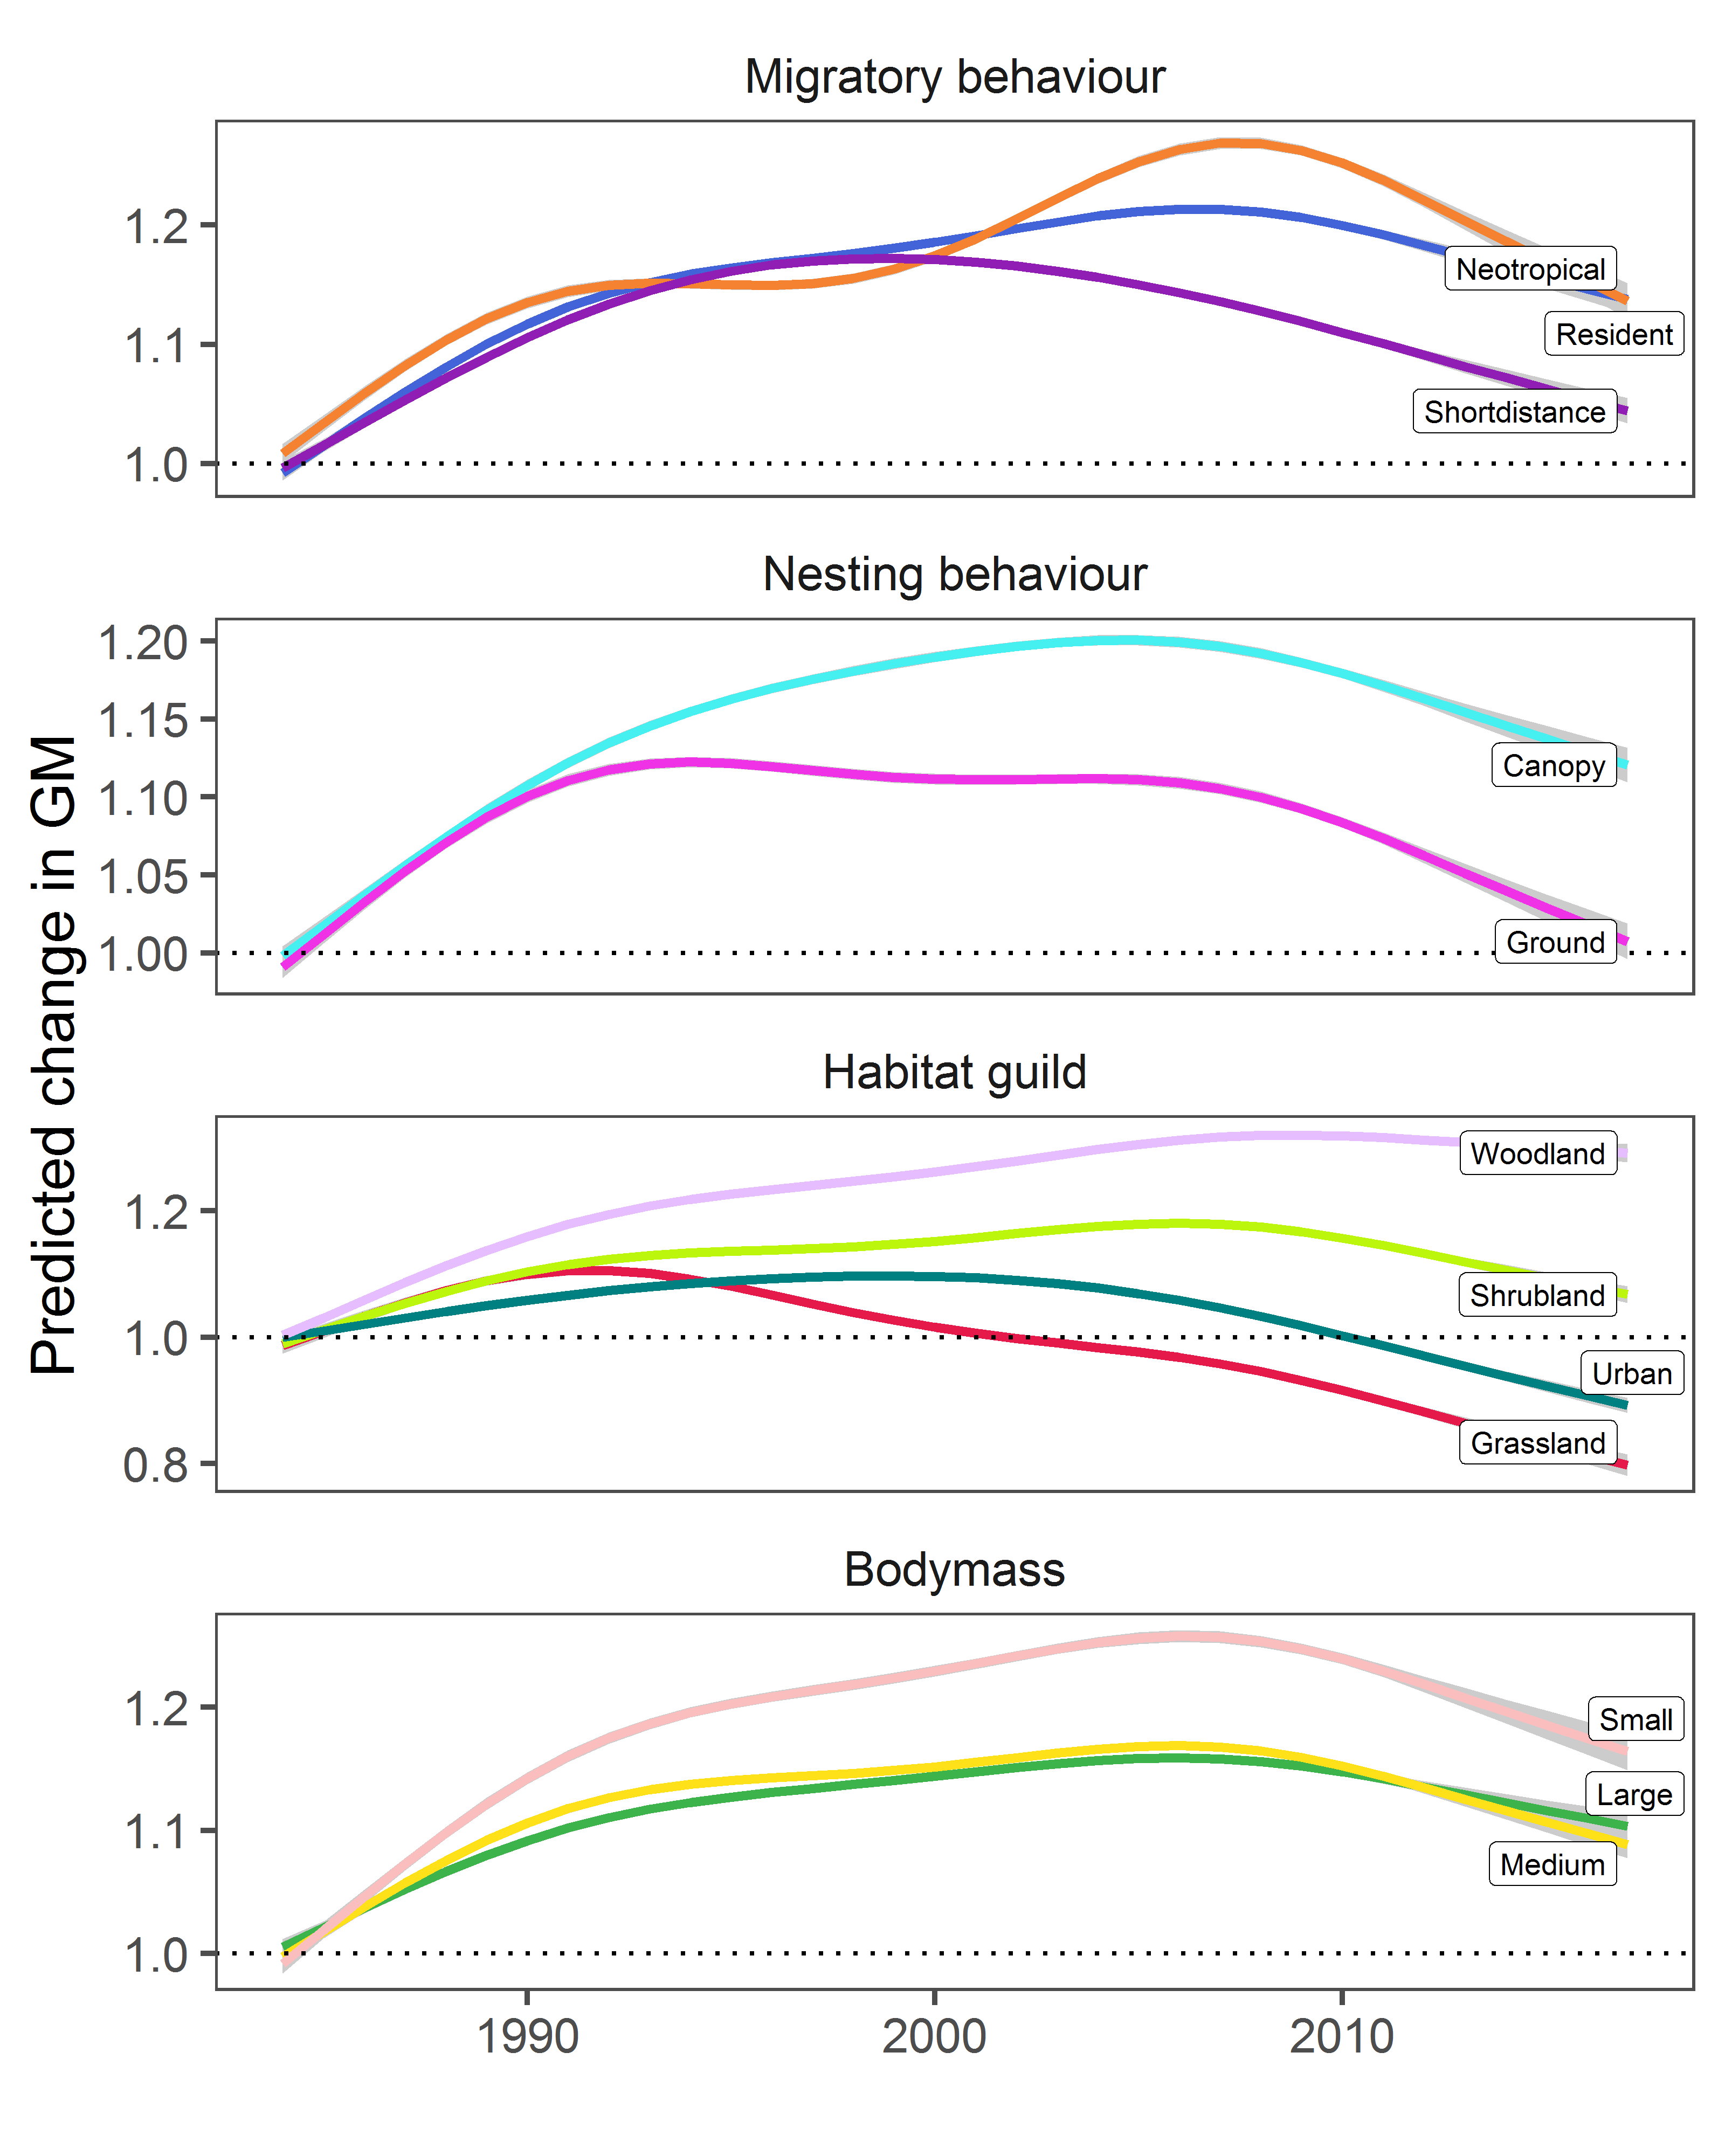
\includegraphics[width=1\textwidth]{chapter5/SI12}
\caption{Change in GM for bird species binned by functional groups of traits. Coloured for better visual distinction only. Error ribbons show the predicted standard error.}
\label{SI05_12}
\end{figure}
